%% ===================================================================
%%  Certified clubs / forgeable greenbeards
%%  SUBMISSION VERSION: Chaos, Solitons & Fractals (Elsevier)
%%
%%  Elsevier CAS bundle, cas-sc.cls = SINGLE COLUMN, which is what the
%%  journal requires of LaTeX submissions.  cas-sc.cls and cas-common.sty
%%  are shipped alongside this file so the source builds anywhere.
%%
%%  Numbered references: the CAS bundle ships only the author-year style
%%  cas-model2-names.bst, so we use Elsevier's numbered-with-names style
%%  elsarticle-num-names.bst, which is what cas-sc's own template points
%%  at when it suggests model1-num-names.
%%
%%  Abstract <= 250 words, highlights 3 to 5 bullets of <= 85 characters,
%%  both also supplied as separate files.
%%
%%    pdflatex main && bibtex main && pdflatex main && pdflatex main
%% ===================================================================
%% longmktitle: the front matter runs past one page, which is exactly
%% what this option is for.
\documentclass[a4paper,fleqn,longmktitle]{cas-sc}

%% Compatibility shim.  cas-common.sty of CAS bundle 2.4 still calls
%% \vbox_unpack_clear:N, which current expl3 releases have removed in favour of
%% \vbox_unpack_drop:N.  Without this, \maketitle fails on an up-to-date TeX
%% installation.  The guard makes it a no-op where the old name still exists.
\ExplSyntaxOn
\cs_if_exist:NF \vbox_unpack_clear:N
  { \cs_new_eq:NN \vbox_unpack_clear:N \vbox_unpack_drop:N }
\ExplSyntaxOff

\usepackage[numbers,sort&compress]{natbib}
\usepackage{amsthm}
\usepackage[section]{placeins}
\usepackage[expansion=false]{microtype}

%% cas-common.sty selects T1 cmss and cmtt for captions, table bodies and
%% \texttt, and no distribution ships those as outlines, so pdflatex embeds
%% six unnamed Type 3 METAFONT bitmaps instead.  A bitmap font carries no
%% usable ToUnicode map, so the ff ligature extracts as U+001B: "payoff"
%% leaves the text layer as "payo" and "first" as "rst".  Latin Modern is the
%% same design with real outlines, so the submitted PDF stays searchable and
%% readable to a screen reader.
\renewcommand{\sfdefault}{lmss}
\renewcommand{\ttdefault}{lmtt}

%% Editorial Manager flattens the upload: the nine figure PDFs arrive next to
%% main.tex with no figures/ directory, while the repository keeps them in
%% one.  Searching both places builds either way.  Deliberately no
%% {thumbnails/} entry: cas-common.sty already asks for
%% thumbnails/cas-email.jpeg, which would then be sought in
%% thumbnails/thumbnails/.
\graphicspath{{figures/}{./}}

\hypersetup{
  allcolors=blue!55!black,
  pdftitle={Forgeable greenbeards: multistability and hollow collapse in certified agent populations},
  pdfauthor={Trung-Kiet Huynh; Dao-Sy Duy-Minh; Chi-Nguyen Tran},
  pdfkeywords={evolutionary game theory; replicator dynamics; multistability; tag-based cooperation; greenbeard; certification; multi-agent systems}
}

% keep floats near the text that refers to them
\renewcommand{\topfraction}{0.92}
\renewcommand{\bottomfraction}{0.75}
\renewcommand{\textfraction}{0.07}
\renewcommand{\floatpagefraction}{0.80}
\setcounter{topnumber}{3}
\setcounter{bottomnumber}{2}
\setcounter{totalnumber}{4}
% a little emergency stretch clears the handful of stubborn lines
\setlength{\emergencystretch}{2em}

\theoremstyle{plain}
\newtheorem{theorem}{Theorem}
\newtheorem{proposition}[theorem]{Proposition}
\newtheorem{lemma}[theorem]{Lemma}
\newtheorem{corollary}[theorem]{Corollary}
\theoremstyle{definition}
\newtheorem{definition}[theorem]{Definition}
\newtheorem{remark}[theorem]{Remark}
%% Two of the numbered statements are computations over sampled initial
%% conditions rather than proofs.  Calling them propositions would promise a
%% proof that the appendix does not contain, so they get their own environment
%% on the shared counter.
\newtheorem{observation}[theorem]{Observation}

\newcommand{\AS}{\textsf{AS}}
\newcommand{\CS}{\textsf{CS}}
\newcommand{\CAS}{\textsf{CAS}}
\newcommand{\AU}{\textsf{AU}}
\newcommand{\piP}{\pi_{P}}
\newcommand{\piS}{\pi_{S}}

\begin{document}
\let\WriteBookmarks\relax
\def\floatpagepagefraction{1}
\def\textpagefraction{.001}

\shorttitle{Forgeable greenbeards}
\shortauthors{T.-K. Huynh et al.}

\title[mode=title]{Forgeable greenbeards: multistability and hollow collapse in
certified agent populations}

%% ------------------------------------------------------------------
%% Chaos, Solitons & Fractals runs a single-anonymized review, so the
%% authors ARE named on the submitted manuscript.  All three contributed
%% equally; the shared first authorship is carried by the
%% \fnmark[1]/\fntext[1] note below.
%% ------------------------------------------------------------------
\author[1]{Trung-Kiet Huynh}[orcid=0009-0000-5463-754X]
\cormark[1]
\fnmark[1]
\ead{23122039@student.hcmus.edu.vn}
\credit{Conceptualization, Methodology, Software, Formal analysis,
Investigation, Validation, Visualization, Writing -- original draft,
Writing -- review and editing}

\author[1]{Dao-Sy Duy-Minh}
\fnmark[1]
\ead{23122041@student.hcmus.edu.vn}
\credit{Conceptualization, Methodology, Software, Formal analysis,
Investigation, Validation, Visualization, Writing -- original draft,
Writing -- review and editing}

\author[1]{Chi-Nguyen Tran}[orcid=0009-0007-6716-7269]
\fnmark[1]
\ead{23122044@student.hcmus.edu.vn}
\credit{Conceptualization, Methodology, Software, Formal analysis,
Investigation, Validation, Visualization, Writing -- original draft,
Writing -- review and editing}

\affiliation[1]{organization={Faculty of Information Technology, University of
            Science, Vietnam National University Ho Chi Minh City},
            addressline={Room I53, Building I, 227 Nguyen Van Cu Street,
            Cho Quan Ward},
            city={Ho Chi Minh City},
            country={Vietnam}}

\cortext[1]{Corresponding author}
\fntext[1]{These authors contributed equally to this work.}

\begin{abstract}
Identity credentials can change how machine agents treat one another, making
them forgeable greenbeards. We study the resulting nonlinear population
dynamics by adding genuine, forged and absent badges to a four-strategy race.
The construction yields 48 designs on a 47-dimensional simplex under
replicator dynamics, with a finite-population counterpart. Most regime
boundaries occur when a transversal eigenvalue changes sign and are therefore
available in closed form; numerical integration is reserved for basin
measures. A reciprocating certified club tolerates more than twice the forgery
of an unconditionally trusting club, so in-group conduct is a security
parameter. The protective fine diverges as forged badges become
undetectable, and verification quality cannot help a costly club nucleate
without positive assortment. At the baseline, a behavioural mimic invades
before an exploiter and hollows out credential integrity while conduct remains
safe. Their invasion boundaries meet at a codimension-two point, beyond which
assortment removes the visible exploiter but not the mimic. Globally, dominant
trajectories converge to disjoint certified and uncertified safe faces, while
targeted starts reach a numerically robust unsafe mixed rest face outside the
uniform sample. Certification therefore
buys robustness to displacement rather than a lower harm level at a settled
state. The same exclusionary conduct that provides this robustness imposes an
entry barrier on compliant unbadged agents; making a club gentle to outsiders
eliminates both the barrier and the club's resistance to forgery.
\end{abstract}

\begin{highlights}
\item A forgeable identity tag induces multistability in a 48-strategy flow
\item Conditional cooperation more than doubles tolerance to credential forgery
\item No finite fine replaces detection as forgery becomes undetectable
\item Mimics hollow out credential integrity before observable conduct degrades
\item Certification buys robustness through an exclusionary entry barrier
\end{highlights}

\begin{keywords}
evolutionary game theory \sep replicator dynamics \sep multistability \sep
tag-based cooperation \sep greenbeard \sep certification \sep
multi-agent systems
\end{keywords}

\maketitle
\section{Introduction}
\label{sec:intro}

Machine agents increasingly carry identity and capability metadata before they
interact~\citep{a2a2026spec}. Regulation already requires providers to identify
AI systems and model versions~\citep{euaiact2024}, while attestation and
provenance infrastructures are being proposed for agent
ecosystems~\citep{chan2024visibility,chan2025infrastructure,shavit2023practices}.
These developments usually frame identity as an accountability tool. Identity
can also change conduct directly: an agent may trust, cooperate with or grant
access to a partner because its credential passes verification.

An identity signal that elicits preferential treatment among its bearers is a
\emph{greenbeard}. Such signals can support cooperation without repeated
interaction, but they fail when the marker separates from the behaviour it is
supposed to identify~\citep{riolo2001evolution,jansen2006altruism,gardner2010greenbeards}.
For machine agents, this separation is an engineering variable rather than a
biological constraint: the pass rate of a forged credential depends on the
verification technology~\citep{jovanovic2024watermarkstealing,anbiaee2026threatmodeling}.
The unresolved question is therefore dynamical. If credentials are costly to
obtain honestly, valuable when accepted and imperfectly verifiable, which
population regimes persist, and how do those regimes change as verification,
penalties and interaction structure vary?

We answer this question by adding a strategic identity layer to a reduced
four-strategy AI race~\citep{domingos2026falling}. Each design combines a badge
that is genuine, forged or absent with conduct toward partners whose badge
passes or fails verification. The construction yields 48 designs evolving on
a 47-dimensional simplex under replicator dynamics; the same payoff structure
also drives a finite-population birth--death process. The underlying race is
held fixed, and every pairwise payoff is evaluated exactly, so all changes are
attributable to the identity layer rather than to sampling or to a modified
interaction game.

The analysis separates local stability from global basin structure. At a
monomorphic resident, invasion is governed by a transversal eigenvalue of the
replicator flow. Most regime boundaries are simple zeros of these eigenvalues
and are therefore available in closed form; numerical integration is used only
to measure basins and to locate attractors. This distinction matters because
the flow is multistable. Averaging states across its disjoint attracting faces
before evaluating a pairwise observable creates cross-regime encounters that
no trajectory contains, so observables must be evaluated within each attractor
and only then averaged over basins.

Three mechanisms organise the results. First, credentials are useful only
where ordinary reciprocity and liability fail to protect safe play. A
reciprocating certified club tolerates more than twice the forgery of an
unconditionally trusting club, showing that in-group conduct is part of the
security design. Penalties help only while detection remains informative: the
protective fine has a vertical asymptote as forged badges become
undetectable. Second, verification does not help a costly club form because an
unbadged population does not read its signal; positive assortment is required
for nucleation. Once formed, however, the club can persist under weaker
conditions than those required to rebuild it after collapse.

Third, certification can fail without an observable deterioration in conduct.
A behavioural mimic copies the club's conduct while avoiding its dues and
crosses its invasion threshold before an exploiter at the baseline. The two
invasion boundaries meet at a codimension-two point, beyond which stronger
assortment removes the visible exploiter while leaving the mimic essentially
unchanged. The credential is then hollow even though behaviour remains safe.
Globally, the dominant trajectories settle on disjoint certified and
uncertified safe faces, while a fully specified targeted start reaches a
numerically robust unsafe mixed rest face outside the uniform sample. Certification
therefore buys robustness to displacement rather than a lower harm level at a
settled state. Its sustaining mechanism is an exclusionary entry barrier: a
club gentle to outsiders is cheaper to imitate and cannot survive forgery.

These results connect nonlinear evolutionary dynamics to certification design.
They also give a practical measurement lesson: conduct alone cannot diagnose
credential integrity. A regime must measure whether passed credentials are
genuine and must treat mutual recognition across providers as part of the
safety architecture, rather than as a separate interoperability choice.
\subsection{Related work}
\label{sec:related}

Evolutionary game dynamics describes a population of competing designs as a
nonlinear flow on a simplex~\citep{taylor1978ess,hofbauer1998evolutionary,hofbauer2003evolutionary}.
Changes in cooperation can then be studied as changes of stability and basin
structure rather than only as changes in an average payoff. Statistical-physics
work on social dilemmas shows that these transitions depend strongly on
interaction structure~\citep{perc2017statphys}; spatial contact, network
heterogeneity and multilayer coupling can each stabilise cooperation
~\citep{nowak1992spatial,santos2005scale,wang2015multilayer}. Recent studies in
\emph{Chaos, Solitons \& Fractals} likewise examine exclusion, tolerance and
evolving reputation as mechanisms that reorganise cooperative
regimes~\citep{ren2021tolerance,zhang2023expulsion,yue2025reputation}. Tags are
one route to assortment without memory, both as phenotypic similarity in a
well-mixed population~\citep{antal2009phenotypic} and as a mutating trait in a
finite population~\citep{traulsen2007chromodynamics}. Our tag differs because
its reliability is a controllable property of a verification technology and
because failure changes which face of the population simplex attracts the
flow.

The biological origin is the greenbeard mechanism: a marker and the behaviour
it elicits are inherited together~\citep{hamilton1964genetical1,dawkins1976selfish}.
Tag similarity can sustain cooperation~\citep{riolo2001evolution}, but
falsebeards profit when the marker separates from the cooperative
behaviour~\citep{jansen2006altruism,gardner2010greenbeards}. Models of
ethnocentrism and parochial altruism also combine an in-group tag with distinct
out-group conduct~\citep{hammond2006ethnocentrism,choi2007parochial}. They rely
on unforgeable or jointly inherited tags, spatial structure or group
competition. Here the tag can be forged at an exogenous pass rate, and
out-group harshness is selected because it makes costly membership excludable,
not because groups fight.

The credential is also a secret handshake: a pre-play signal that a mutant may
display without the conduct it advertises~\citep{robson1990efficiency}.
Classical signalling models maintain honesty through differential costs
~\citep{grafen1990biological,spence1973job}; certification intermediaries
instead disclose otherwise hidden quality~\citep{dranove2010quality}. Our
forger pays less than a compliant member, so honesty rests on imperfect
detection. Penalties and detection are normally substitutes
~\citep{becker1968crime}; the model identifies where that substitution fails
when detection is fixed by technology.

Finally, evolutionary models of AI races have studied regulation, voluntary
commitments, auditing and trust~\citep{han2020regulate,han2022voluntary,bova2024vigilant}.
Agent-governance work treats identity, visibility and provenance as
prerequisites~\citep{chan2024visibility,chan2025infrastructure,otsuka2026aiidentity},
while empirical work documents identity-conditioned evaluation and imperfect
model-origin recognition~\citep{panickssery2024llm,sun2025idiosyncrasies,wang2026outgroup}.
Those literatures do not derive the population-level consequences of a
credential that is both valuable and worth forging. The present model supplies
that link through local bifurcation thresholds and global basin analysis.
\section{Model}
\label{sec:model}

\subsection{The interaction layer}
\label{sec:race}

The interaction layer is the reduced race of~\citet{domingos2026falling},
reproduced without modification. Two seats repeatedly choose Safe or Unsafe.
Unsafe pays more in the stage game and advances the race faster, but accumulates
private setback risk for whoever leads at the horizon. The horizon is
stochastic: $T = 5 + G$ with $G$ geometric at rate $0.2$, so $\mathbb{E}[T] = 9$.
Four reduced designs are considered, in increasing order of the harm they cause:
\AS{} is always safe, \CS{} opens safe and mirrors, \CAS{} opens unsafe and
mirrors, and \AU{} is always unsafe.

Because the four designs are deterministic, the action path of an ordered pair
is fixed once the pair is fixed, and every matchup is evaluated by exact
expectation over the horizon law rather than by sampling. We write $A$ for the
$4 \times 4$
matrix of expected race payoffs, $M$ for the expected number of Unsafe actions
of the focal seat, and $U$ for the expected fraction of Unsafe rounds;
Table~\ref{tab:race} gives $A$ and $M$.

\subsection{The identity layer}
\label{sec:identity}

Each seat is operated by an agent that carries a badge and conditions its
conduct on the badge its partner
presents~\citep{long2025mirror,wang2026outgroup}. A design is a triple
$(b, s_{\mathrm{in}}, s_{\mathrm{out}})$ with $b \in \{\mathsf{G}, \mathsf{F},
\mathsf{N}\}$ and $s_{\mathrm{in}}, s_{\mathrm{out}}$ reduced race designs, so
the design space has $3 \times 4 \times 4 = 48$ elements. We call a design
carrying $b = \mathsf{F}$ a \emph{falsebeard}~\citep{gardner2010greenbeards},
and one carrying $b = \mathsf{G}$ a \emph{certified club} whatever its conduct
pair; the club $(\mathsf{G}, \CS, \CAS)$ that dominates the results below is
the \emph{baseline club}.

A badge either passes a verification check or does not. Missing mandatory
validation or attestation is a documented security risk in agent
protocols~\citep{anbiaee2026threatmodeling}. We represent that risk by letting a
genuine badge always pass, an absent badge never pass, and a forged badge pass
with probability $\sigma$, the \emph{spoof success probability}; $1 - \sigma$
is the detection power of the attestation technology. Verification happens once, at
the start of a race, and holds for its duration. That matches the interaction
layer, in which the executed design of a seat is fixed before the first round.
The check is the secret handshake of~\citet{robson1990efficiency} with a failure
rate attached: a pre-play signal that selects which conduct each seat executes,
and that a mutant can display without the conduct behind it.
The two checks of an encounter concern two different badges, so they are
independent by construction, and every pairwise expectation is an exact
four-term sum,
\begin{equation}
\label{eq:handshake}
a(i, j) \;=\; \sum_{\substack{x \in \{\mathrm{in}, \mathrm{out}\} \\
                              y \in \{\mathrm{in}, \mathrm{out}\}}}
  w_x(q_j)\, w_y(q_i)\; A\big(s^{i}_{x},\, s^{j}_{y}\big),
\qquad
w_{\mathrm{in}}(q) = q, \quad w_{\mathrm{out}}(q) = 1 - q,
\end{equation}
where $q_i$ is the rate at which design $i$'s badge elicits the in-group
response. The harm matrix $m(i,j)$ and the behaviour matrix $u(i,j)$ are the
same sum with $M$ and $U$ in place of $A$.

Carrying a badge costs something. A genuine badge costs $\kappa_g$ per race,
the price of issuance, attestation and compliance; a forged badge costs
$\kappa_f$, and the interesting regime is $\kappa_f < \kappa_g$. A detected
forgery may additionally be fined $\rho$, so a forger expects to pay
$(1 - \sigma)\rho$ per encounter.

Detection has two consequences that the model keeps separate, because they are
different instruments. Under \emph{screening} the checking agent responds to a
failed badge by playing $s_{\mathrm{out}}$: verification happens in real time
and the counterparty can act on it. Under \emph{retrospective auditing} the
fine is levied but the behavioural response is not available, because the
detection arrives after the interaction; formally, $q_{\mathsf{F}} = 1$ while
the expected fine is still $(1 - \sigma)\rho$. Section~\ref{sec:channels}
separates the two.

Finally, agents do not meet uniformly at random. With probability $r$ an agent
interacts within its own provider cluster, modelled as meeting its own
design~\citep{grafen1979hawk},
and with probability $1 - r$ it meets a uniform draw from the population. This
is the one parameter the identity layer does not create: it is the pre-existing
structure of the agent economy, in which agents of one provider co-occur on one
platform.

\subsection{Two functionals}
\label{sec:functionals}

The \emph{private} functional is what the operator of a seat receives,
\begin{equation}
\label{eq:private}
\piP(i, j) \;=\; a(i, j) \;-\; L\, m(i, j) \;-\; c(b_i) \;-\; f(b_i),
\end{equation}
with $L$ the liability charged per Unsafe action of one's own seat, $c$ the
badge cost and $f$ the expected fine. The \emph{social} functional counts the
full harm and the real resource costs, but not fines, which are transfers:
\begin{equation}
\label{eq:social}
\piS(i, j) \;=\; a(i, j) \;-\; h\, m(i, j) \;-\; c(b_i).
\end{equation}
Here $h$ is the social cost of one unsafe action, so $\piS$ charges the full
harm rather than the share attributable to any one seat.
Only $\piP$ drives the dynamics; $\piS$ is the yardstick. The baseline sets
$L = 0$. That setting is the regime the paper is about: where harm cannot be
attributed to the seat that caused it, the liability channel is
closed~\citep{chan2024visibility,kolt2025governing} and identity is the only
channel left. Section~\ref{sec:liability} reopens it and measures what
identity is worth as a function of $L$.

\subsection{Dynamics, observables and parameters}
\label{sec:dynamics}

We report two dynamics because they answer two different questions about the
same game. The finite-population pairwise-comparison process in the
small-mutation limit~\citep{fudenberg2006imitation,traulsen2006stochastic}
answers which single design the market spends its time in, since under rare
mutation the population is monomorphic almost always. The replicator
flow~\citep{taylor1978ess,hofbauer1998evolutionary}, run from many interior
initial conditions, answers a different question: from an arbitrary starting
composition, which regime does the market settle into, and how large is each
basin. Both act on the assortment-adjusted private functional. The replicator
flow is integrated with EGTtools~\citep{domingos2023egttools}; the
small-mutation chain uses a closed-form birth-death fixation probability,
which is what makes the 48-design space tractable, and is checked against the
full EGTtools chain on reduced spaces.

Everything else in the study is evaluated exactly; the replicator basins are
the only sampled quantities, and there are four families of them. Interior
starts are drawn $\mathrm{Dirichlet}(1, \dots, 1)$ on the simplex under a fixed
seed: $20\,000$ starts for the headline split of
Observation~\ref{prop:bistable}, and $200$ each for every out-group conduct of
Table~\ref{tab:outgroup}, for every fine level of
Corollary~\ref{cor:rescue} and at each verification level of the agreement
check in Section~\ref{sec:robustness}. A basin share is a sample proportion, so
the headline one is reported with a Wilson interval; the $200$-start shares
carry a standard error near $0.035$ and are quoted to one digit accordingly.


\paragraph{The flow.}
Write $\Delta$ for the simplex of population states over the $48$ designs and
$x \in \Delta$ for a state. With assortment $r$, the expected private payoff of
design $i$ is
\begin{equation}
\label{eq:fitness}
f_i(x) \;=\; r\,\piP(i,i) \;+\; (1-r)\sum_{j} x_j\, \piP(i,j),
\end{equation}
and the replicator flow is
\begin{equation}
\label{eq:replicator}
\dot{x}_i \;=\; x_i\big[\,f_i(x) - \bar{f}(x)\,\big],
\qquad \bar{f}(x) \;=\; \sum_k x_k f_k(x).
\end{equation}
Every vertex $e_j$ of $\Delta$ is a rest point of
Equation~\eqref{eq:replicator} at every parameter value, and the eigenvalue of
the linearisation at $e_j$ transversal to that vertex in the direction of
design $i$ is
\begin{equation}
\label{eq:eigen}
\lambda_{i \mid j} \;=\; f_i(e_j) - f_j(e_j)
  \;=\; r\,\piP(i,i) \;+\; (1-r)\,\piP(i,j) \;-\; \piP(j,j).
\end{equation}
Each $\lambda_{i \mid j}$ is affine in the fine $\rho$, in the badge costs
$\kappa_g$ and $\kappa_f$, in the liability $L$ and in the assortment $r$,
because the functional of Equation~\eqref{eq:private} is affine in each of
them. In the spoof success $\sigma$ it is affine only where the handshake is
evaluated on at most one forged badge. Equation~\eqref{eq:handshake} is affine
in each pass rate separately but \emph{bilinear} in the pair, so a term in
which both seats carry forged badges contributes a $\sigma^{2}$, and
Equation~\eqref{eq:eigen} contains such a term whenever the invader is a
badge-conditional forger meeting itself under assortment, or invader and
resident are both forgers. Of the thresholds reported below, exactly one is
affected: at $r = 0.1$ the mimic's eigenvalue is
$-0.2075\,\sigma^{2} + 32.5075\,\sigma - 30.300$, whose only root in $[0,1]$ is
$\sigma_m = 0.9377$, the other lying at $155.7$. Every threshold reported in
Section~\ref{sec:results} is therefore the unique root in $[0,1]$ of one such
eigenvalue in one parameter, and is available in closed form either way.

The qualitative event each threshold marks is a transcritical
bifurcation~\citep{strogatz2018nonlinear} of the flow restricted to the
edge $\{e_i, e_j\}$, on which Equation~\eqref{eq:replicator} reduces to
$\dot{x} = x(1-x)\,[\,f_i(x) - f_j(x)\,]$ with the bracket affine in $x$ at
fixed parameters: writing it as $\alpha + \beta x$, the interior edge
equilibrium sits at $-\alpha/\beta$ with $\alpha = \lambda_{i \mid j}$, so it
passes through the vertex exactly as the eigenvalue changes sign and exchanges
stability with it. The two conditions this needs hold at every threshold we
report. Transversality is the requirement that the eigenvalue cross with
non-zero speed in its parameter, which the closed forms below exhibit
directly; non-degeneracy is the requirement $\beta \neq 0$, and the values are
$2.48$ and $-0.70$ on the exploiter edge at $r = 0$ and $r = 0.1$, $-0.0079$
and $-0.0072$ on the mimic edge, $-2.08$ on the reciprocity edge and $29.80$
on the nucleation edge. On the mimic edge $\beta$ is small, so the interior
equilibrium traverses the edge within a $\sigma$ window of order
$10^{-4}$ and the exchange is sharp in practice as well as in principle. This
is why the thresholds below are exact rather than estimated, and it is what the
closed forms in Section~\ref{sec:results} are expressions for.

The distinction between the two dynamics is not a robustness check, and it
needs one
piece of care that is easy to skip. The replicator flow of this game turns out
to be multistable, with attractors on disjoint faces of the simplex
(Observation~\ref{prop:bistable}). Every observable here is bilinear in the
population state, so evaluating one at the arithmetic mean of two disjoint
attractors invents encounters between designs that never actually meet. We
therefore evaluate every observable \emph{at each attractor} and average the
results over basins, never the reverse. Section~\ref{sec:exclusion} reports
what the two conventions differ by, because the gap is large enough to change
the sign of a headline effect.

Beyond the population unsafe frequency $U$ and the social payoff, we report
three observables specific to the identity layer. The \emph{attestation
integrity} is the posterior $\Pr(\text{badge genuine} \mid \text{badge
passed})$, the epistemic content of a passed check. The \emph{mark lift} is
$\Pr(\text{partner behaves safely} \mid \text{its badge passed}) -
\Pr(\text{partner behaves safely} \mid \text{it did not})$, the behavioural
value of a passed check to the agent that performed it. The \emph{harm
decomposition} assigns every ordered encounter to one of four blocks by the
badge status of the two seats and splits $U$ across them exactly.

Baseline parameters are $\sigma = 0.5$, $\kappa_g = 2$ (about $3.5\%$ of the
$57.0$ a safe club member nets), $\kappa_f = 0$ (forgery is free, the worst
case), $\rho = 0$ (fines are an instrument, not part of the world), $r = 0.1$,
$L = 0$, $h = 20$, population size $Z = 100$ and selection intensity
$\beta = 0.05$. Every one of them is swept.

% generated by scripts/build_paper.py -- do not edit
\begin{table}[pos=t]
\centering
\caption{The interaction layer, exactly evaluated over the horizon
law: expected race payoff $A$ (left) and expected number of unsafe
actions $M$ (right) of the row design against the column design.
The row that drives every result is \CAS{} against \CS{}: a first
strike earns $61.63$ where the resident earns $59.00$ against itself, at the cost of $4.78$ unsafe actions, so reciprocity deters it
only above $L_R = 0.551$.}
\label{tab:race}
\small
\begin{tabular}{lrrrrcrrrr}
\toprule
 & \multicolumn{4}{c}{payoff $A$} & & \multicolumn{4}{c}{unsafe actions $M$} \\
\cmidrule{2-5}\cmidrule{7-10}
 & AS & CS & CAS & AU & & AS & CS & CAS & AU \\
\midrule
AS & 59.00 & 59.00 & 8.60 & 5.40 & & 0.00 & 0.00 & 0.00 & 0.00 \\
CS & 59.00 & 59.00 & 26.64 & 16.60 & & 0.00 & 0.00 & 4.22 & 8.00 \\
CAS & 101.77 & 61.63 & 27.20 & 27.20 & & 1.00 & 4.78 & 9.00 & 9.00 \\
AU & 48.64 & 47.36 & 27.20 & 27.20 & & 9.00 & 9.00 & 9.00 & 9.00 \\
\bottomrule
\end{tabular}
\end{table}

\begin{table}[pos=t]
\centering
\caption{Closed-form thresholds of the identity layer at zero
liability.  $\sigma^{*}$ is the spoof success above which the
unconditional forger invades the certified reciprocator club and
$\sigma_m$ the threshold for the behavioural mimic, both evaluated
in a well-mixed population; $r^{*}$ is itself an assortment, the one
below which no club nucleates whatever the verification.  Note that
$\sigma_m$ exceeds $\sigma^{*}$ in every row: well mixed, the
exploiter invades first.  The order reverses above $r = 0.077$
(Section~\ref{sec:mimicry}), which is why the baseline $r = 0.1$ has
$\sigma^{*} = 0.962 > \sigma_m = 0.938$ and why the manuscript
reports the mimic as the first invader.  Dues weaken the club; fines
strengthen it only through the detections the screen already makes.}
\label{tab:thresholds}
\small
\begin{tabular}{rrrrr}
\toprule
dues $\kappa_g$ & fine $\rho$ & $\sigma^{*}$ (forger) & $\sigma_m$ (mimic) & $r^{*}$ \\
\midrule
0.5 & 0 & 0.909 & 0.985 & 0.016 \\
0.5 & 5 & 0.921 & 0.987 & 0.016 \\
0.5 & 20 & 0.942 & 0.990 & 0.016 \\
1.0 & 0 & 0.895 & 0.969 & 0.031 \\
1.0 & 5 & 0.908 & 0.973 & 0.031 \\
1.0 & 20 & 0.933 & 0.981 & 0.031 \\
2.0 & 0 & 0.866 & 0.938 & 0.063 \\
2.0 & 5 & 0.883 & 0.946 & 0.063 \\
2.0 & 20 & 0.915 & 0.962 & 0.063 \\
4.0 & 0 & 0.807 & 0.876 & 0.126 \\
4.0 & 5 & 0.832 & 0.893 & 0.126 \\
4.0 & 20 & 0.878 & 0.924 & 0.126 \\
8.0 & 0 & 0.691 & 0.753 & 0.252 \\
8.0 & 5 & 0.730 & 0.786 & 0.252 \\
8.0 & 20 & 0.805 & 0.847 & 0.252 \\
\bottomrule
\end{tabular}
\end{table}

\begin{table}[pos=t]
\centering
\caption{The baseline equilibrium across nested design pools, in the
small-mutation limit ($\sigma = 0.5$, $r = 0.1$, $\kappa_g = 2$,
$L = 0$, $Z = 100$, $\beta = 0.05$).  The identity layer roughly
halves the long-run unsafe frequency of the uncertified world;
forgery at a coin-flip spoof rate claws back about a quarter of the
gain that unforgeable badges would deliver.}
\label{tab:pools}
\small
\begin{tabular}{lrrrrr}
\toprule
design pool & unsafe & club & falsebeard & integrity & social \\
\midrule
certified world (48 designs) & 0.090 & 0.42 & 0.07 & 0.92 & 39.1 \\
unforgeable badges (32) & 0.068 & 0.47 & 0.00 & 1.00 & 43.6 \\
uncertified world (16) & 0.159 & 0.00 & 0.00 & 1.00 & 25.4 \\
raw race (4) & 0.159 & 0.00 & 0.00 & 1.00 & 25.4 \\
\bottomrule
\end{tabular}
\end{table}

\begin{table}[pos=t]
\centering
\caption{The symmetric $K$-provider world under provider-scoped
marks.  Cross-provider checks fail, so the ecosystem unsafe
frequency is $1 - \mathrm{HHI}$ exactly; federated recognition
plays the club design throughout and is safe at any concentration.
The exclusion rent is the payoff gap between a member and a
compliant unbadged entrant.}
\label{tab:providers}
\small
\begin{tabular}{rrrrrr}
\toprule
$K$ & HHI & unsafe (scoped) & unsafe (federated) & member & rent \\
\midrule
1 & 1.000 & 0.000 & 0.000 & 57.0 & 30.4 \\
2 & 0.500 & 0.500 & 0.000 & 41.1 & 14.5 \\
3 & 0.333 & 0.667 & 0.000 & 35.8 & 9.2 \\
4 & 0.250 & 0.750 & 0.000 & 33.2 & 6.5 \\
8 & 0.125 & 0.875 & 0.000 & 29.2 & 2.5 \\
20 & 0.050 & 0.950 & 0.000 & 26.8 & 0.1 \\
\bottomrule
\end{tabular}
\end{table}


\section{Results}
\label{sec:results}


Table~\ref{tab:bifurcations} maps the qualitative changes analysed below to
their control parameters and locations.

\begin{table}[pos=t]
\centering
\caption{Qualitative transitions of the identity layer. Rows one to four and
six are edge transcritical bifurcations; row five is the codimension-two
intersection of two such bifurcation curves. Row seven is the vertical
asymptote of a marginal-stability locus, and row eight is a global basin
property.}
\label{tab:bifurcations}
\small
\vspace{2pt}
\begin{tabular}{@{}p{5.6cm}p{2.2cm}lp{3.6cm}@{}}
\toprule
transition & parameter & location & value \\
\midrule
safe unbadged resident loses stability to a first-striker
  & liability $L$
  & Eq.~\eqref{eq:LR}
  & $L_R = 0.551$ \\[2pt]
certified club loses stability to an unconditional forger
  & spoof success $\sigma$
  & Eq.~\eqref{eq:sigmastar}
  & $\sigma^{*} = 0.866$ at $r = 0$, $0.962$ at $r = 0.1$ \\[2pt]
certified club loses stability to a behavioural mimic
  & spoof success $\sigma$
  & Eq.~\eqref{eq:sigmam}
  & $\sigma_m = 0.938$ \\[2pt]
unbadged resident loses stability to a certified club
  & assortment $r$
  & Eq.~\eqref{eq:rstar}
  & $r^{*} = 0.063$ \\[2pt]
the two invading eigenvalues vanish together and the invaders exchange order
  & $(r, \sigma)$ jointly
  & Eq.~\eqref{eq:sigmastar}, \eqref{eq:sigmam}
  & $r = 0.077$ \\[2pt]
the forger's threshold leaves the admissible range of $\sigma$
  & assortment $r$
  & Eq.~\eqref{eq:sigmastar}
  & $r = 0.134$ \\[2pt]
the locus of marginal protection escapes to infinity
  & $(\sigma, \rho)$ jointly
  & Eq.~\eqref{eq:rhostar}
  & pole at $\sigma \to 1$ \\[2pt]
two measure-dominant rest faces in the uniform-start experiment
  & none
  & Obs.~\ref{prop:bistable}
  & shares $0.388$, $0.612$; targeted unsafe face outside sample \\
\bottomrule
\end{tabular}
\end{table}

Proofs of all propositions appear after the main text. The two
statements labelled as observations are computations over sampled initial
conditions rather than proofs, and are labelled that way for exactly that
reason.

\subsection{Why identity is needed: the reciprocity threshold}
\label{sec:reciprocity}

The race has a property that decides what any identity layer has to do. Consider
a population of unbadged reciprocators, all playing \CS{}: open safe, then
mirror. A rare \CAS{} mutant opens unsafe, takes a half-step lead in the first
round, and is mirrored from the second round onwards. Reciprocity punishes it,
but only in kind, and the stolen half-step survives to the horizon and converts
into the prize. The mutant earns $61.63$ against the resident's $59.00$, at the
cost of $4.78$ extra unsafe actions.

\begin{proposition}[Reciprocity threshold]
\label{prop:reciprocity}
At zero assortment, the advantage of the first-striker is affine in liability
and vanishes at
\begin{equation}
\label{eq:LR}
L_R \;=\; \frac{A(\CAS, \CS) - A(\CS, \CS)}{M(\CAS, \CS) - M(\CS, \CS)}
      \;=\; 0.551 .
\end{equation}
For the canonical safe unbadged resident whose out-group conduct is \CS{}, the
joint invasion advantage is
\begin{equation}
\label{eq:jointfirststrike}
\Delta(L,r) = 2.631 - 34.431r - (4.78 + 4.22r)L .
\end{equation}
The first-striker invades precisely when $\Delta(L,r)>0$. Thus
$L_R=0.551$ and $r^{\dagger}=0.076$ are the intercepts $L_R(0)$ and
$r^{\dagger}(0)$, not independent bounds defining a rectangle. At $L=0$,
the unbadged first-striker $(\mathsf{N}, \CAS, \CAS)$ invades every unbadged
resident that plays safe conduct in self-play, where
\begin{equation}
\label{eq:rdagger}
r^{\dagger} \;=\; \frac{A(\CAS, \CS) - A(\CS, \CS)}{A(\CAS, \CS) - A(\CAS, \CAS)}
      \;=\; 0.076 .
\end{equation}
At $r=0$, no unbadged population sustains safe play for $L<L_R$, whatever its
conduct rule; at other $(L,r)$ values this conclusion must be checked against
the joint boundary in Equation~\eqref{eq:jointfirststrike}.
\end{proposition}

Both bounds are needed, and the second is as informative as the first. The
first-striker's transversal eigenvalue at a safe unbadged resident is
$A(\CAS, \CS) - A(\CS, \CS) - r\,[A(\CAS, \CS) - A(\CAS, \CAS)]
 = 2.631 - 34.431\,r$: clustering makes a first-striker meet its own aggression,
and by $r^{\dagger} = 0.076$ that self-encounter has eaten the whole stolen
half-step. Above $r^{\dagger}$ the four residents $(\mathsf{N}, \cdot, \CS)$
resist it, which is why the uncertified regime of
Observation~\ref{prop:bistable} is a safe one even at $L = 0$. The proposition
is checked exhaustively over the eight safe unbadged residents rather than
argued. Its content is that within-race reciprocity is not enough on its own:
the race rewards the opening move, a mirror cannot undo an opening move, and
what rescues a safe unbadged population is the very assortment that
Section~\ref{sec:nucleation} shows a club also needs. Something outside the
race must distinguish partners before the first round, and that is what a badge
does.

Figure~\ref{fig:handshake}B shows the consequence. At $L = 0$ and no
assortment, the uncertified world runs at unsafe frequency $1.000$: it is
complete anarchy. The value of identity is therefore not a marginal
improvement on a functioning market. It is the difference between a market and
no market. Conversely, once $L$ rises above $L_R$ the liability channel does
the work by itself, and Section~\ref{sec:liability} shows the identity layer
becoming worthless there.

\begin{figure}[pos=t]
\centering
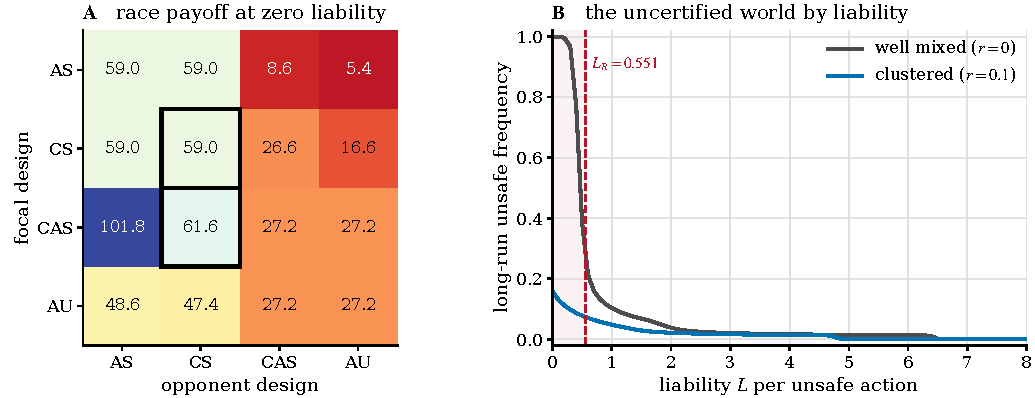
\includegraphics[width=\linewidth]{figures/fig02_handshake.pdf}
\caption{\textbf{The race rewards the opening move, so reciprocity alone cannot
hold a safe population.} \textbf{(A)} Private race payoff $A - LM$ at $L = 0$.
The boxed cells are the handshake exploit: a \CAS{} first-striker earns $61.63$
against a \CS{} resident that earns $59.00$ against itself. \textbf{(B)}
Long-run unsafe frequency of the uncertified world (badge $\mathsf{N}$ only) as
liability rises. The shaded region is $L < L_R = 0.551$, where
Proposition~\ref{prop:reciprocity} rules out any safe unbadged population in a
well-mixed one. Without clustering the world is fully unsafe there; the
clustered baseline sits above $r^{\dagger} = 0.076$, so some safe unbadged
residents survive, and it is better but still far from safe.}
\label{fig:handshake}
\end{figure}

\subsection{How much forgery a club survives}
\label{sec:spoof}

A certified club is a design $(\mathsf{G}, u, v)$: carry a genuine badge, play
$u$ towards partners whose badge passes, $v$ towards everyone else. A forger
$(\mathsf{F}, w, \cdot)$ buys access to the in-group conduct $u$ with
probability $\sigma$ and pays $\kappa_f$ rather than $\kappa_g$.

\begin{proposition}[Spoof threshold]
\label{prop:spoof}
For an unconditional forger $(\mathsf{F}, w, w)$ against a club
$(\mathsf{G}, u, v)$ in a well-mixed population, the invasion condition is
affine in $\sigma$ and the threshold is
\begin{equation}
\label{eq:sigmastar}
\sigma^{*} \;=\;
  \frac{P(u,u) - P(w,v) - \kappa_g + \kappa_f + \rho}
       {P(w,u) - P(w,v) + \rho},
\qquad P = A - L M .
\end{equation}
Provided $P(w,u) - P(w,v) + \rho > 0$, the club resists forgery for all
$\sigma < \sigma^{*}$. When that denominator is negative the invasion advantage
decreases in $\sigma$ and the inequality reverses, so the club resists only
above $\sigma^{*}$; when it vanishes, which happens exactly when
$\rho=P(w,v)-P(w,u)$ (within the feasible domain $\rho\geq 0$), the
forger's advantage is the constant
$P(w,u) - P(u,u) + \kappa_g - \kappa_f$, independent of $\sigma$ altogether.
\end{proposition}

Equation~\eqref{eq:sigmastar} says something that is not obvious in advance:
the club's in-group conduct enters the threshold twice, once through what
members earn among themselves, $P(u,u)$, and once through what an impostor
extracts from them, $P(w,u)$. A club whose members trust unconditionally
maximises the second term, and so minimises its own tolerance for forgery. In a
well-mixed population the reciprocating club $(\mathsf{G}, \CS, \CAS)$ survives
up to $\sigma^{*} = 0.866$; the unconditionally trusting club
$(\mathsf{G}, \AS, \CAS)$ survives only to $0.400$. At the baseline assortment
$r = 0.1$ the pair is $0.962$ against $0.444$, because a forger's
self-encounters are worth much less to it than a member's are. The ratio is
$2.17$ at both, so it is the conduct and not the structure that sets it.
Membership conduct is a security parameter.

The sign condition of Proposition~\ref{prop:spoof} is not a technicality, and
Section~\ref{sec:exclusion} is where it does its work: the denominator
$P(w,u) - P(w,v) + \rho$ is positive for a club that treats outsiders harshly
and non-positive for one that does not, so the two gentle out-group policies
have no threshold to report rather than a low one.
Figure~\ref{fig:invasion} shows the invasion advantage as a function of
$\sigma$ in both structures, and the fixation probabilities that the
finite-population process assigns to the same invasions.

\begin{figure}[pos=t]
\centering
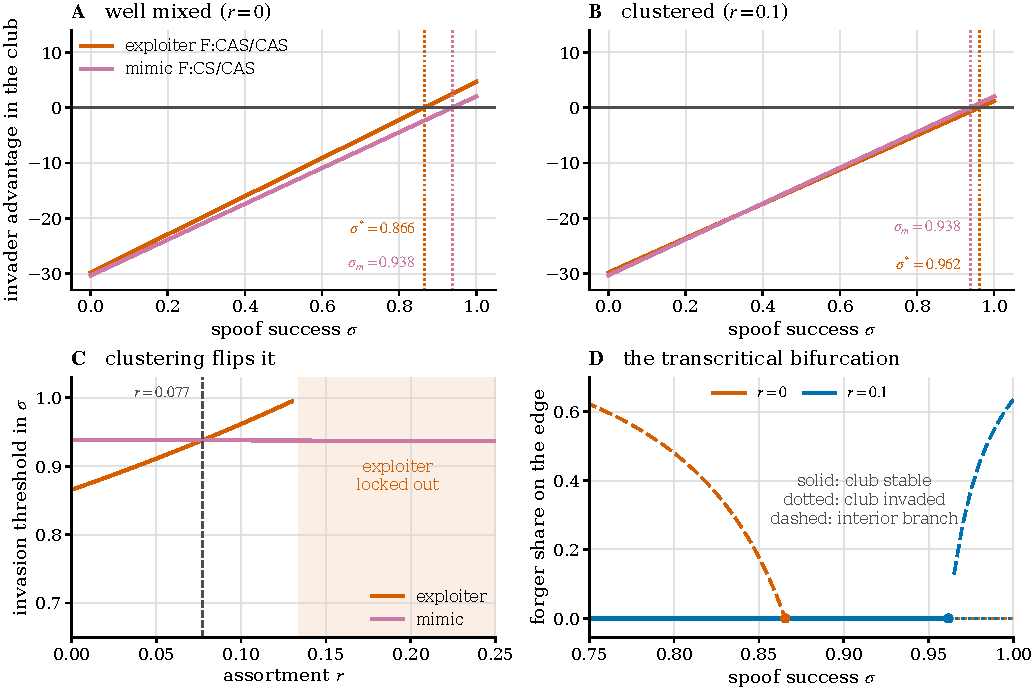
\includegraphics[width=\linewidth]{figures/fig03_invasion.pdf}
\caption{\textbf{Clustering decides which of the two invaders reaches the club
first.} Advantage of a rare invader in a monomorphic club
$(\mathsf{G}, \CS, \CAS)$, \textbf{(A)} well mixed and \textbf{(B)} at the
baseline assortment $r = 0.1$; dotted verticals mark the thresholds, whose
values are printed because a gap of $0.024$ is not legible on a unit axis.
\textbf{(C)} The same two thresholds against assortment. Clustering raises the
exploiter's threshold steeply and leaves the mimic's flat, so the two cross at
$r = 0.077$ and the exploiter is locked out entirely above $r = 0.134$. Better
interaction structure removes the visible failure mode and not the invisible
one. \textbf{(D)} The bifurcation the first three panels locate, drawn on the
$\{$club, exploiter$\}$ edge. The horizontal branch is the club vertex, solid
where it resists invasion and dotted where it does not; the dashed branch is
the interior edge equilibrium $-\alpha/\beta$ of
$\dot{x} = x(1-x)(\alpha + \beta x)$. The two exchange stability where they
meet, at $\sigma^{*} = 0.866$ well mixed and $0.962$ at the baseline
assortment: a transcritical bifurcation, and the reason every threshold in
Table~\ref{tab:bifurcations} is a simple root rather than an estimate.}
\label{fig:invasion}
\end{figure}

\subsection{Fines cannot buy what detection does not deliver}
\label{sec:fines}

A natural response to forgery is to punish it. Setting the invasion advantage
to zero and solving for the fine gives the break-even protective penalty.

\begin{proposition}[Becker limit of attestation]
\label{prop:fines}
In a well-mixed population, the break-even fine against the unconditional
forger is
\begin{equation}
\label{eq:rhostar}
\rho^{*}(\sigma) \;=\;
  \frac{\sigma\,[P(w,u) - P(w,v)] - [P(u,u) - P(w,v)] + \kappa_g - \kappa_f}
       {1 - \sigma},
\end{equation}
which diverges as $\sigma \to 1$ whenever exploiting the club at full pass
beats club membership. Where the club already resists unaided, that is for
$\sigma < \sigma^{*}$, the expression is negative and the smallest feasible
fine is $\max\{0,\rho^{*}(\sigma)\}$.
\end{proposition}

The expected penalty a forger faces is $(1 - \sigma)\rho$, so as detection power
vanishes the fine required to maintain a fixed expected penalty grows without
bound. The divergence is the Becker trade-off between penalty size and
detection probability~\citep{becker1968crime,polinsky2000economic}, and the
numbers are stark: well mixed, $\rho^{*} = 11.9$ at $\sigma = 0.90$, $58.2$ at
$0.95$ and $428.6$ at $0.99$, against a club payoff of $57.0$. Beyond about
$\sigma = 0.95$ the fine needed exceeds everything the club is worth. Assortment
does not remove the pole, it only moves where it starts to bite: at the
baseline $r = 0.1$ the club resists the exploiter unaided up to
$\sigma^{*} = 0.962$, so nothing is required below that, and the requirement is
then $8.6$ at $\sigma = 0.97$ and $87.8$ at $\sigma = 0.99$. What the model
determines robustly is the divergence; where a given regime sits on the curve
depends on its interaction structure.

The novelty is not the trade-off but which of its terms is available. In
conventional enforcement the detection probability is bought with inspectors,
so a regulator facing a high cost of detection can substitute a higher penalty
and reach the same deterrence. Here the detection probability is a property of
the attestation technology, and a regime that has deployed a weak one cannot
buy its way out with penalties. The fine here is levied by an authority rather
than by peers, so it escapes the second-order free-rider problem that
constrains punishment in evolutionary settings where the punishing itself is
costly and voluntary~\citep{szolnoki2017second}; what constrains it instead is
detection alone. Figure~\ref{fig:instruments}B shows the divergence.

Dues run the other way, and the closed form makes the direction unconditional.
Differentiating Equation~\eqref{eq:sigmastar},
\begin{equation}
\label{eq:duesgrad}
\frac{\partial \sigma^{*}}{\partial \kappa_g}
  \;=\; \frac{-1}{P(w,u) - P(w,v) + \rho} \;=\; -0.029
\end{equation}
at the baseline, so every unit of certification cost lowers the club's forgery
tolerance. Compliance cost burdens the compliant and never the impostor by
construction, so every unit lowers forgery tolerance. This cost allocation is a
modelling assumption, distinct from the information and intermediary-incentive
problems studied in the certification literature~\citep{dranove2010quality}.
Table~\ref{tab:thresholds} sweeps the dues against the fine and shows the
two moving in opposite directions across the whole grid.
The remedy is not cheaper dues but dearer forgery: raising $\kappa_f$ increases
$\sigma^{*}$ with slope $1/[P(w,u)-P(w,v)+\rho]$, which is $+0.029$ at the
baseline, and Figure~\ref{fig:instruments}D shows it working
at a spoof rate where nothing else does.

\begin{figure}[pos=t]
\centering
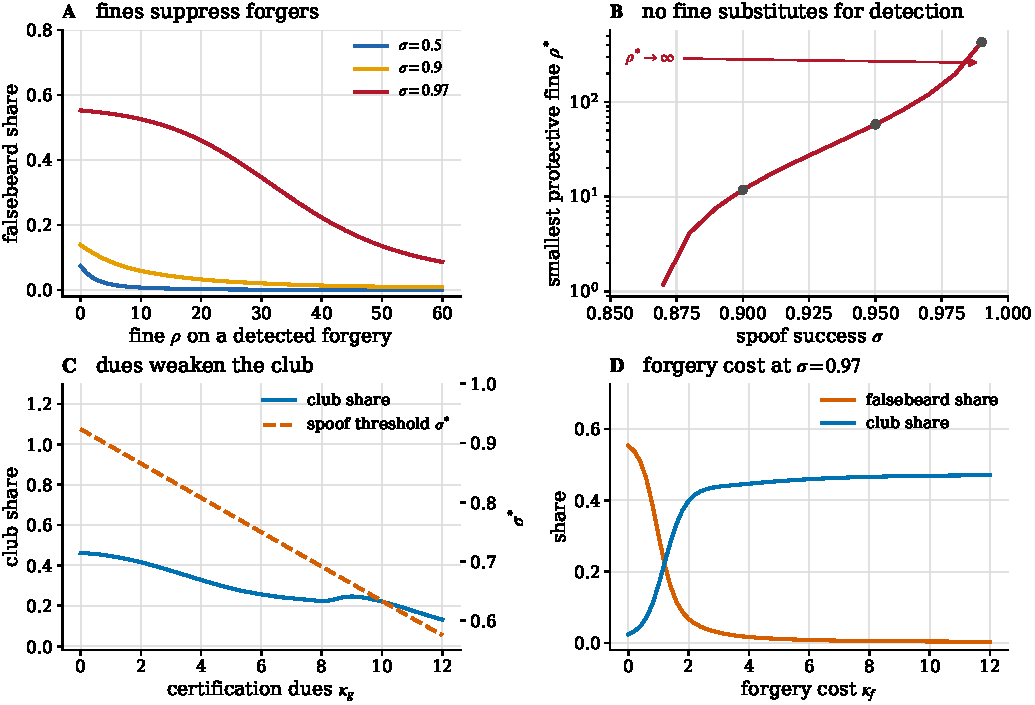
\includegraphics[width=\linewidth]{figures/fig06_instruments.pdf}
\caption{\textbf{Four instruments, three of which have a limit.}
\textbf{(A)} Fines suppress forgers, and less so as detection weakens.
\textbf{(B)} The break-even protective fine diverges as $\sigma \to 1$
(Proposition~\ref{prop:fines}); note the logarithmic axis. \textbf{(C)}
Certification dues weaken the club on both margins: the club share falls and
the spoof threshold falls with it, by Equation~\eqref{eq:duesgrad}.
\textbf{(D)} Raising the cost of forgery is the one cost-side instrument that
burdens the impostor rather than the member, shown at $\sigma = 0.97$ where
the club would otherwise be extinct.}
\label{fig:instruments}
\end{figure}

\subsection{No badge starts a club by itself}
\label{sec:nucleation}

Everything above concerns a club that already exists. Whether one can form is a
separate question with a blunt answer.

\begin{proposition}[Badge futility]
\label{prop:futility}
Against any resident whose conduct does not condition on badges, a certified
design earns exactly its unbadged twin's payoff minus the dues, at every
$\sigma$, every $\rho$ and every $L$. Consequently, at $r = 0$ and
$\kappa_g > 0$, no certified design invades any unconditional resident that its
unbadged twin could not already invade.
\end{proposition}

The reason is that a badge is a signal, and a signal changes nothing when
nobody reads it~\citep{katz1985network}. A club must therefore bootstrap from encounters with itself,
which is what assortment supplies.

\begin{proposition}[Nucleation threshold]
\label{prop:nucleation}
Against an unconditional unbadged resident $(\mathsf{N}, w, w)$ with
$P(u,u) > P(v,w)$, a club $(\mathsf{G}, u, v)$ invades exactly when
\begin{equation}
\label{eq:rstar}
r \;>\; r^{*} \;=\; \frac{P(w,w) - P(v,w) + \kappa_g}{P(u,u) - P(v,w)}
  \;=\; 0.063
\end{equation}
at the baseline, where the denominator is
$P(\CS,\CS) - P(\CAS,\CAS) = 31.80$. The hypothesis is not decoration: the
inequality is the sign of that denominator, and when it is negative assortment
obstructs the club rather than enabling it. Against the \emph{safe} unbadged
resident $(\mathsf{N}, \CS, \CS)$ the denominator is $-2.63$ and the baseline
club invades only \emph{below} $r = 0.240$. When it vanishes the club invades
at no assortment at all.
\end{proposition}

The two residents are the two regimes of Observation~\ref{prop:bistable}, so
the reversal is the statement that nucleating a club out of anarchy and
nucleating one out of a settled safe uncertified market are different problems
with opposite comparative statics in the one instrument available. Assortment
is what lets a club form in an anarchic market, and it is also what lets a safe
unbadged market resist one.

Taken together the two propositions say that verification quality and
assortment are not substitutes. Attestation engineering, however good, moves
$\sigma$, and $\sigma$ does not appear in Equation~\eqref{eq:rstar}. What does
appear is the dues, which is why a certification regime that is expensive to
join can be unable to start even when it would be stable once running.
Figure~\ref{fig:nucleation} shows the phase structure: panel A the switch at
$r^{*}$, panel B the two-dimensional region in which a club can live, and
panel C the asymmetry between keeping a club and building one.

That asymmetry is the sixth result. At $r = 0$ a club cannot re-enter a
population that has collapsed either to forgery or to anarchy, at any $\sigma$
whatsoever: the re-entry threshold does not exist. The conditions for holding a
certification regime together are strictly weaker than the conditions for
assembling one, so a regime that is allowed to collapse is not recovered by
restoring the policy that sustained it.

\begin{figure}[pos=t]
\centering
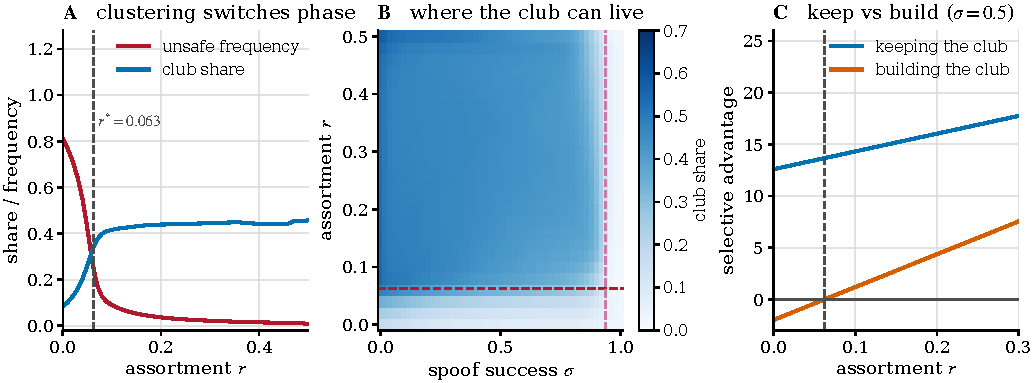
\includegraphics[width=\linewidth]{figures/fig05_nucleation.pdf}
\caption{\textbf{Clubs need clustering, and losing one is worse than never
having had it.} \textbf{(A)} Unsafe frequency and club share against
assortment; the club switches on at $r^{*} = 0.063$
(Proposition~\ref{prop:nucleation}). \textbf{(B)} Club share over spoof success
and assortment. The horizontal line is $r^{*}$ and the vertical line is the
mimicry threshold $\sigma_m$; the club lives in the region between them.
\textbf{(C)} The advantage of holding a club against forgery (blue) exceeds the
advantage of building one from anarchy (orange) at every assortment, and the
gap is what makes collapse irreversible.}
\label{fig:nucleation}
\end{figure}

\subsection{Collapse hollows out the mark before it degrades the conduct}
\label{sec:mimicry}

Proposition~\ref{prop:spoof} concerns a forger that exploits. A different
invader is available, and it arrives first. The \emph{mimic}
$(\mathsf{F}, u, v)$ plays exactly the club's conduct and differs only in
carrying a forged badge. It free-rides on the dues, not on the behaviour.

\begin{proposition}[Mimicry threshold]
\label{prop:mimicry}
In the well-mixed limit $r=0$, the behavioural mimic invades the club when
\begin{equation}
\label{eq:sigmam}
\sigma \;>\; \sigma_m \;=\; 1 - \frac{\kappa_g - \kappa_f}{P(u,u) - P(u,v) + \rho}
  \;=\; 0.938 ,
\end{equation}
At the baseline assortment $r=0.1$, the exact invasion advantage is instead
quadratic in $\sigma$ and its relevant root is $\sigma_m=0.9377$; it still lies
below the exploiter's threshold $0.9617$.
\end{proposition}

The ordering of the two thresholds is not fixed, and what moves it is the one
instrument that otherwise looks unambiguously good. Assortment penalises an
exploiter, because an exploiter meets its own aggressive conduct in a
self-encounter, and does not penalise a mimic, because a mimic meets the club's
conduct, which is what a mimic plays. The exploiter's threshold therefore
climbs from $0.866$ at $r = 0$ to $1$ by $r = 0.134$, beyond which no forgery
quality whatsoever lets an exploiter in, while the mimic's threshold moves by
$0.001$ across the entire range. They cross at $r = 0.077$
(Figure~\ref{fig:invasion}C), where the two codimension-one bifurcation
curves meet transversally in the $(r, \sigma)$ plane. Both transversal
eigenvalues of Equation~\eqref{eq:eigen} at the club vertex vanish there, and
because the transversal block of the Jacobian at a vertex is diagonal those
zeros are semisimple: $(r, \sigma) = (0.077, 0.938)$ is a codimension-two
point at which two independent transcritical events coincide, not a degenerate
singularity with a normal form of its own. What changes as the point is
crossed is only which of the two the ecosystem meets first. The club vertex is
in any case never hyperbolic: inside a monomorphic club every check passes,
$s_{\mathrm{out}}$ is never executed, and the seven other designs
$(\mathsf{G}, u, v)$ with $u \in \{\AS, \CS\}$ are payoff-equivalent to
it, so seven transversal eigenvalues vanish identically at every parameter
value. The
exchange of stability is therefore a statement about the invading edge and not
about the vertex as a whole.

The consequence is uncomfortable for the instrument of
Section~\ref{sec:nucleation}. Clustering is what makes clubs possible at all,
and it is also what removes the visible failure mode that conduct monitoring
can see among the sampled invaders. Past $r = 0.134$ the remaining route
identified in this analysis is impersonation
by an agent that behaves correctly, so the better the interaction structure,
the more completely the residual risk is concentrated in the failure that looks
like success.

Between the two thresholds the ecosystem behaves well and means nothing. At
$\sigma = 0.96$, which lies inside the baseline window $(0.938, 0.962)$,
forgers hold $0.54$ of the population, the certified club has
fallen to $0.04$, the unsafe frequency is $0.063$ against the baseline $0.090$,
and the posterior probability that a passed badge was actually issued has
fallen to $0.07$. An observer monitoring conduct would report that the
certification regime is working, and would read the improvement in unsafe
frequency as evidence for it. An observer asking what a certificate certifies
would find that it certifies nothing.

Figure~\ref{fig:cliff} traces the whole sweep. The composition in panel A
shifts from the certified club to the falsebeard class as $\sigma$ crosses
$\sigma_m$. Panel C separates the two things a passed check could be worth: the
attestation integrity falls through one half at $\sigma = 0.93$, while the mark
lift, the behavioural value of a passed check, turns negative already at
$\sigma = 0.57$. That inversion is worth stating plainly. Beyond $\sigma =
0.57$ a partner whose badge passes your check is \emph{less} likely to treat
you safely than one whose badge fails, because passing is what the exploiters
do. The check has become an anti-signal~\citep{harbaugh2011label}. We are careful not to overstate what
follows. The certified world still has a lower unsafe frequency than the
uncertified world at every $\sigma$ (Figure~\ref{fig:cliff}B), so verification
is not worse than nothing in aggregate. What is worse than nothing is the
\emph{advice} a passed check gives an individual agent, which above
$\sigma = 0.57$ points towards the partners least deserving of trust. A
protocol that instructs agents to extend credit on a passed credential is, in
that regime, instructing them wrongly.

\begin{figure}[pos=t]
\centering
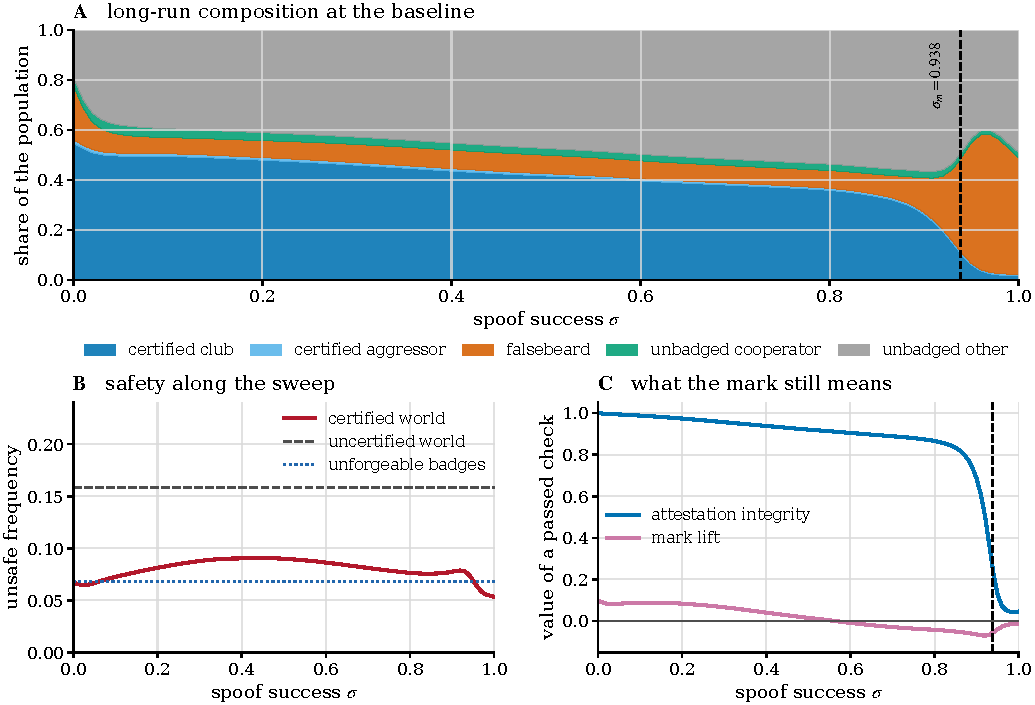
\includegraphics[width=\linewidth]{figures/fig04_cliff.pdf}
\caption{\textbf{The certification cliff.} \textbf{(A)} Long-run composition
against spoof success; the dashed line is the mimicry threshold $\sigma_m =
0.938$. \textbf{(B)} Unsafe frequency of the certified world against the
uncertified world and against a counterfactual in which badges cannot be
forged. \textbf{(C)} The two things a passed check can be worth. Attestation
integrity, the posterior that a passed badge is genuine, survives until
$\sigma_m$; the mark lift, the behavioural value of a passed check, is already
negative at $\sigma = 0.57$.}
\label{fig:cliff}
\end{figure}

\subsection{Screening and fining are different instruments}
\label{sec:channels}

One detection has two consequences, and governance regimes choose between them
without always noticing. Real-time verification lets the counterparty act on a
failed check; retrospective auditing levies a fine after the fact. The
$2 \times 2$ of Figure~\ref{fig:channels} switches each off in turn at
$\sigma = 0.9$ and $\rho = 20$.

The placebo cell, in which badges are checked but nothing follows from a failed
check, leaves attestation integrity at $0.05$: the population is essentially
all forgers. Screening alone raises it to $0.68$ and fines alone to $0.53$;
together they reach $0.94$. The two channels are complements rather than
substitutes, and neither reaches on its own what both reach together, which runs
against the penalty-detection substitution of the standard enforcement
model~\citep{becker1968crime,polinsky2000economic}.

The unsafe frequency tells a different story from the integrity, and this is
the point of separating them. Across the four cells $U$ moves only between
$0.053$ and $0.077$, while integrity moves from $0.05$ to $0.94$. An evaluation
regime that monitors conduct would rate all four cells as roughly equivalent
and would be unable to distinguish a working attestation system from a
completely hollow one. Attestation integrity has to be measured directly.

\begin{figure}[pos=t]
\centering
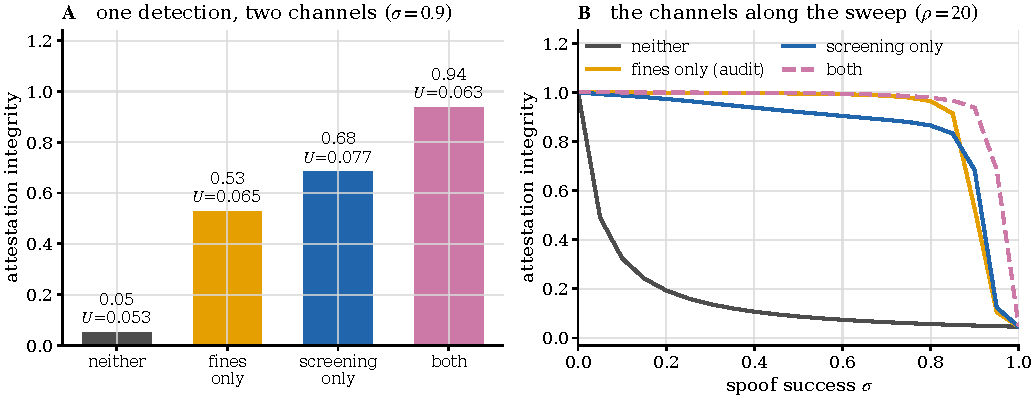
\includegraphics[width=\linewidth]{figures/fig07_channels.pdf}
\caption{\textbf{The two consequences of one detection.} \textbf{(A)}
Attestation integrity in the $2 \times 2$ at $\sigma = 0.9$, $\rho = 20$, with the
unsafe frequency of each cell printed above the bar. Integrity varies by a
factor of nearly twenty across cells in which the unsafe frequency barely
moves. \textbf{(B)} The same four regimes along the spoof sweep.}
\label{fig:channels}
\end{figure}

\subsection{Provider-scoped marks make concentration a safety variable}
\label{sec:providers}

Current agent-identity approaches use incompatible credential formats, trust
roots and delegation semantics~\citep{otsuka2026aiidentity}. We model one
plausible consequence: marks issued per provider need not be recognised by
another provider. Consider $K$
symmetric provider clubs, each running the club design with its own mark, with
cross-provider checks failing by construction.

\begin{proposition}[Concentration frontier]
\label{prop:providers}
With symmetric shares the within-provider encounter probability equals the
Herfindahl index $\mathrm{HHI} = 1/K$, and the ecosystem unsafe frequency is
\begin{equation}
\label{eq:hhi}
U \;=\; \mathrm{HHI}\; U(u,u) \;+\; (1 - \mathrm{HHI})\; U(v,v)
  \;=\; 1 - \mathrm{HHI}
\end{equation}
for the baseline club. Under federation, in which marks are mutually
recognised~\citep{nicolaidis2005transnational}, the ecosystem plays $u$ throughout
and $U = 0$ at any
concentration.
\end{proposition}

A duopoly runs at $U = 0.500$ and eight providers at $0.875$
(Table~\ref{tab:providers}). Read naively this
is an argument for concentration, which is not the reading we intend. It is an
argument that scoping a safety mark to an issuer converts market structure into
a safety variable, and that federation removes the dependence entirely.

The obstacle is that the incentive to federate runs backwards.
Figure~\ref{fig:providers}B shows the exclusion rent, the payoff gap between a
club member and a compliant unbadged entrant that plays club conduct towards
everyone and is treated as an outsider by every club. The rent is $30.4$ under
a single club and $2.5$ across eight. A dominant provider therefore has the
most to lose from mutual recognition~\citep{katz1985network}, and a fragmented
market has the least to gain from it while needing it most. The exclusion rent
is also a competition concern in its own right: in the model, a compliant
entrant is penalised $30.4$ under a monopoly mark for no reason connected to
its conduct. This is the kind of entry barrier that equitable-interoperability
proposals seek to reduce~\citep{scottmorton2023equitable}.

\begin{figure}[pos=t]
\centering
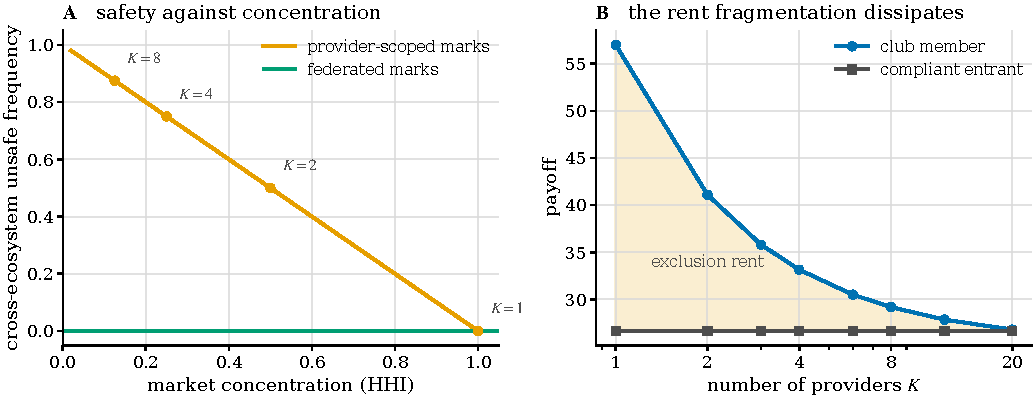
\includegraphics[width=\linewidth]{figures/fig08_providers.pdf}
\caption{\textbf{Scoped marks tie safety to market structure.} \textbf{(A)}
Cross-ecosystem unsafe frequency against concentration under provider-scoped
marks is exactly $1 - \mathrm{HHI}$; federated marks are safe at any
concentration. \textbf{(B)} The exclusion rent, the payoff gap between a club
member and a compliant unbadged entrant, dissipates as the market fragments,
so the provider best placed to federate is the one least willing to.}
\label{fig:providers}
\end{figure}

\subsection{Multistability, and where the exclusion is actually paid}
\label{sec:exclusion}

The results so far read as a qualified endorsement of certification: it works,
it has thresholds, and the thresholds can be engineered. The eighth result
qualifies the endorsement in a way that the thresholds do not reveal.

The long-run composition summaries above use the small-mutation limit, which
describes a market that is monomorphic almost always and moves between designs
by mutation and fixation; the local invasion thresholds and payoff identities
are exact and do not rely on that limit. The replicator flow asks a different
question: from an arbitrary
starting composition, what does the market settle into? The answer is not one
thing.

\begin{observation}[Dominant two-face split and a targeted unsafe rest face, numerical]
\label{prop:bistable}
At the baseline, no interior start in the uniform Dirichlet sample reached a
badge-mixed rest point. Of $20\,000$ such starts, $38.8\%$ converged to a state
that is entirely badged and $61.2\%$ to one that is entirely unbadged (Wilson
$95\%$ interval $[38.2, 39.5]$ on the first), and no design has positive growth
at any end state reached. Both regimes are internally safe: the largest unsafe
frequency over all end states is below $10^{-13}$.
A deterministic targeted start places $0.70$ on $(\mathsf{F},\AU,\AU)$ and
spreads the remaining mass uniformly across the other 47 designs. It reaches
an unsafe badge-mixed rest state with $U=1.000$, badged mass $0.937$, field
residual below $10^{-13}$ and no design with invasion growth above $10^{-13}$.
All $64$ deterministic full-dimensional perturbations
$x_0^{(k)}=0.95x_0+0.05z_k$, with $z_k\sim\operatorname{Dirichlet}(1)$ under
the recorded seed, also reach $U=1.000$ and have no invasion growth above
$10^{-13}$. This finite neighbourhood probe shows numerical robustness, not
the basin's volume or a third isolated attractor. The reported two-face split
is therefore measure-specific and does not establish global bistability.
\end{observation}

Figure~\ref{fig:exclusion}A plots a readable subsample of the uniform starts,
all of them landing on one of the two pure regimes.

The limit sets deserve their proper names, because the flow is more degenerate
than ``two attractors'' suggests. Inside a certified population every check
passes, so $s_{\mathrm{out}}$ is never executed and the eight designs
$(\mathsf{G}, u, v)$ with $u \in \{\AS, \CS\}$ all earn exactly $57.0$; inside
an uncertified population no check ever passes, so $s_{\mathrm{in}}$ is never
executed and the survivors all earn $59.0$. Each regime is therefore not an
isolated point but a face of the simplex carrying a continuum of neutrally
stable rest points, and the $20\,000$ runs reach $20\,000$ distinct ones. What
is bistable is the pair of faces, not a pair of equilibria. Neither face is
attracting in its entirety either: the attracting part is cut out by the
condition that no design outside it can grow, and a certified composition
weighted far enough towards gentle out-group conduct falls outside and drains
to the uncertified regime instead.

That degeneracy is worth naming rather than hiding, because it says something
about the mechanism. The out-group coordinate is \emph{exactly} neutral inside
a settled certified regime: a club never meets an outsider there, so nothing
selects what it would do if it did. The composition of any one certified rest
point is a memory of the transient that produced it, not a selected state, and
the club $(\mathsf{G}, \CS, \CAS)$ holds $0.83$ of the certified face on
average across end states while ranging over almost the whole unit interval.
Out-group harshness is load-bearing where selection can see it, in the invasion
thresholds of Equation~\eqref{eq:sigmastar} and Table~\ref{tab:outgroup}, and
inert at the rest point itself. The uncertified regime is dominated in the same
average sense by the first-striker $(\mathsf{N}, \CAS, \CS)$, at $0.71$.

Both regimes look unsafe by name and neither is: inside a certified regime
every member runs \CS{} against every partner it meets, and inside an
uncertified regime every design runs its out-group conduct, which for the
survivors is \CS{}. Each population has selected a conduct that is safe against
the only partner it ever meets.

Two caveats on the quantifier, both of which a reader reproducing this should
know. The first is that $38.8\%$ is a property of the starting measure and not
of the flow: it is the share of the uniform Dirichlet draining to the certified
face, and a more concentrated start measure gives a different number. At $200$
draws, which is what a sweep can afford, the sampling error on it is about
$0.035$, so only the first digit is real. The second is that ``no badge-mixed
rest point'' is a statement about what the sample reached, not a theorem. Other
rest points exist and the uniform measure does not find them. The targeted
experiment in Observation~\ref{prop:bistable} reaches a maximally unsafe mixed
rest face and survives the recorded finite perturbation probe. That evidence
does not establish the face's basin volume or justify calling it a third
isolated attractor. The two-face split we report is therefore explicitly a
property of the uniform-start experiment.

The coincidence of the two safe regimes has an immediate and unflattering
consequence for certification.

\begin{corollary}[No safety dividend on the dominant safe faces]
\label{cor:dues}
Since both dominant faces are safe, the social payoff of the certified regime differs
from the uncertified one only by the certification cost: $57.0$ against
$59.0$, a gap of $2.0 = \kappa_g$ to machine precision. Conditional on
convergence to either dominant safe face, the identity layer buys no safety
and costs exactly its dues.
\end{corollary}

The small-mutation result of Section~\ref{sec:results} is not contradicted by
this, and putting the two together is the point. Under rare mutation the
certified world runs at $0.090$ against the uncertified $0.159$, so
certification does reduce harm there. What it reduces is not the harm of a
settled market, which is zero either way, but the harm the market suffers while
being knocked out of safety and finding its way back. Certification buys
\emph{robustness}, not \emph{level}. A regulator who measures a running,
undisturbed ecosystem will find the certified and uncertified versions equally
safe and the certified one poorer by its dues, and will be measuring the wrong
thing.

\paragraph{Where the exclusion is.}
The club that survives is the one whose conduct towards outsiders is \CAS{},
and the natural expectation is that the resulting harm shows up in encounters
between the two regimes. Observation~\ref{prop:bistable} rules that out: in
equilibrium the two regimes do not meet, so no such encounters occur. The
exclusion is real all the same, and it is paid as a barrier rather than as a
running harm.

\begin{proposition}[The entry barrier]
\label{prop:exclusion}
Let a compliant outsider be an unbadged design that plays the club's own
in-group conduct towards everybody, so that it is behaviourally beyond
reproach. Every club member's check of it fails, so every member executes its
out-group conduct against it. Against the surviving club
$(\mathsf{G}, \CS, \CAS)$, well mixed, the outsider earns $26.64$ where a member
nets $57.00$, a penalty of $30.36$ for no conduct-related reason, and the
encounter runs at unsafe frequency $0.461$; at the baseline assortment the
penalty is $27.12$. Against a gentle club
$(\mathsf{G}, \CS, \CS)$ the penalty is $-2.00$ at either assortment: the
outsider is \emph{better off} than the member, by exactly the dues, and the
encounter is entirely safe.
\end{proposition}

One thing this quantity is not. Certification is available in the model at
$\kappa_g = 2$, and $(\mathsf{G}, \CS, \CAS)$ is one of the $48$ designs, so
$30.36$ is not a price of admission that an outsider is prevented from paying.
It is the selection pressure the club exerts on a design that declines to pay
it, which is the same thing seen from the other side: it is what holds the club
together, and what an unbadged incumbent gives up by staying outside. That is
still an entry barrier in the sense that matters for competition policy, since
it is a payoff gap imposed for carrying no badge rather than for conduct, but
it is not a wall.

The two halves of Proposition~\ref{prop:exclusion} are the whole argument,
and Figure~\ref{fig:exclusion} shows both: panel B the dues-sized payoff gap
between the two settled regimes, panel C the toll ordering that
Table~\ref{tab:outgroup} tabulates.

Table~\ref{tab:outgroup} scans the four possible out-group policies and the
ordering is exact. The two gentle policies, \AS{} and \CS{}, impose an entry
penalty of $-2.00$ and a boundary unsafe frequency of $0$; both have spoof
threshold exactly $0$ and equilibrium share $0.02$ or less. The two harsh
policies, \CAS{} and \AU{}, impose penalties of $30.36$ and $40.40$ and
boundary unsafe frequencies of $0.461$ and $0.868$; both have spoof threshold
$0.962$ and take essentially the whole population under rare mutation. Nothing
in between appears, because a club that is gentle to outsiders has made its
badge behaviourally empty, at which point the dues buy nothing and any forger
saves them.

\begin{table}[pos=t]
\centering
\caption{The out-group policy of a certified club decides both what it
tolerates and what it costs an outsider. Each row restricts the design pool to
one certified design plus every unbadged and forged design. The entry penalty
is the payoff gap between a member and a compliant unbadged entrant that plays
the club's own conduct towards everyone; the boundary unsafe frequency is what
that encounter runs at. The two policies that impose no barrier are exactly the
two that cannot survive forgery.}
\label{tab:outgroup}
\small
\begin{tabular}{lrrrrr}
\toprule
conduct towards & spoof threshold & entry & boundary & club share & certified \\
outsiders & $\sigma^{*}$ & penalty & unsafe & (monomorphic) & basin \\
\midrule
\AS{}  & 0.000 & $-2.00$ & 0.000 & 0.005 & 0.000 \\
\CS{}  & 0.000 & $-2.00$ & 0.000 & 0.020 & 0.000 \\
\CAS{} & 0.962 & $30.36$ & 0.461 & 1.000 & 0.885 \\
\AU{}  & 0.962 & $40.40$ & 0.868 & 1.000 & 0.395 \\
\bottomrule
\end{tabular}
\end{table}

There is an obvious objection, and answering it sharpens the result rather than
softening it. If the problem is that a gentle club gives an impostor nothing to
lose, then supply the loss externally: fine detected forgery, and the badge
becomes worth acquiring honestly again. The first half of that works.

\begin{corollary}[A fine restores the barrier, not the purpose]
\label{cor:rescue}
A fine on detected forgery raises the gentle club's spoof threshold from
exactly $0$ at $\rho = 0$ to $0.923$ at $\rho = 60$, so forgery no longer
defeats it. Its equilibrium share nonetheless never exceeds $0.032$ at any fine
level tested, in either reading of the dynamics.
\end{corollary}

The reason is Proposition~\ref{prop:futility}. A fine changes what a forger
faces; it does not change what a badge earns against residents who do not read
badges. A gentle certified club is behaviourally indistinguishable from the
unbadged cooperator $(\mathsf{N}, \CS, \CS)$, which supplies the same conduct
without the dues, so the club is dominated whatever the fine. Resistance to
forgery and a reason to exist are separate requirements, and out-group
harshness is the only conduct in this game that supplies both. What the fine
does buy is worth stating, since the corollary is not an argument for doing
nothing: it raises attestation integrity from $0.16$ to $0.98$ and lifts the
social payoff of the full design space from $39.1$ to $43.6$. It makes the
credential meaningful. It does not make the gentle club exist.

It is worth being precise about what carries the result, because a reader who
knows the parochial-altruism literature will expect a different mechanism.
\citet{choi2007parochial} obtain a similar inseparability from group selection:
hostility is favoured because it produces the intergroup conflicts in which
in-group altruism pays. Nothing of that kind is present here. There are no
groups that compete, no conflict whose outcome anyone wins, and no selection
above the level of the individual design. What drives our version is
excludability. The dues $\kappa_g$ are a real cost, and a club that treats
outsiders exactly as it treats members converts its badge into a label that
predicts nothing about conduct, so the dues purchase nothing and the cheapest
way to carry the badge is to forge it. Equation~\eqref{eq:sigmastar} shows this
directly: when $u = v$ the denominator $P(w,u) - P(w,v) + \rho$ collapses to
$\rho$, so at $\rho = 0$ the forger's advantage does not depend on $\sigma$ at
all and is positive because the forger saves the dues. Out-group harshness is
the only thing that makes the in-group benefit excludable. In this model it
raises the potential cost of cheating relative to honest acquisition, the kind
of off-equilibrium cost that can maintain honesty without a realised
equilibrium signal cost~\citep{szamado2011cost}.

\paragraph{A note on how not to compute this.}
An earlier version of this analysis averaged the replicator attractors into a
single state and evaluated the observables there. Every observable in this
model is bilinear in the population state, so scoring one at the mean of two
disjoint attractors invents encounters between designs that never meet: the
mean of the certified and uncertified faces assigns $47.5\%$ of encounters to
badged-unbadged pairs and reports an unsafe frequency of $0.368$, when every
rest point being averaged has zero such encounters and an unsafe frequency below
$10^{-13}$. The error is easy to make and hard to see, because the mean state
is a perfectly valid probability vector. We report it here because the
corrected reading is the more interesting one, and because a reader comparing
against a multistable model of their own should know which of the two
quantities they are looking at.

\begin{figure}[pos=t]
\centering
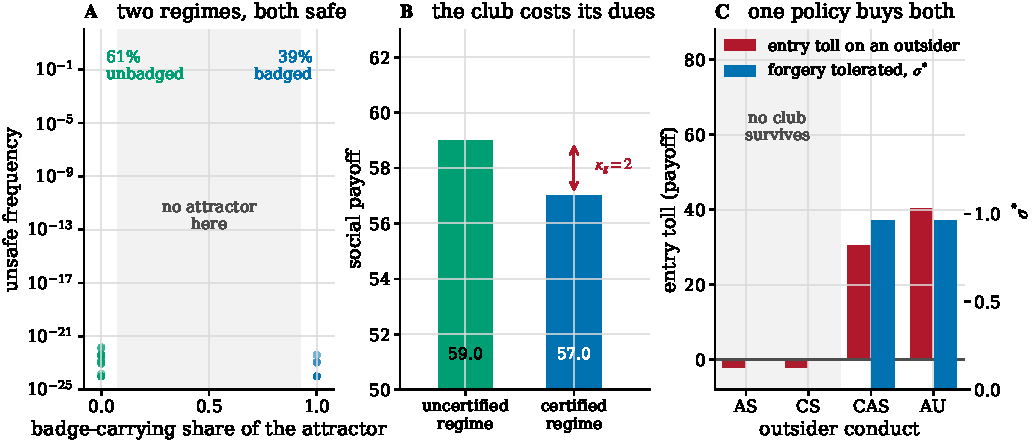
\includegraphics[width=\linewidth]{figures/fig01_exclusion.pdf}
\caption{\textbf{The market settles into one of two internally safe regimes,
and the cost of certification is a barrier at the boundary rather than harm
inside it.} \textbf{(A)} Each of the $200$ interior starts plotted here, a
readable subsample of the $20\,000$ behind
Observation~\ref{prop:bistable}, reaches a pure regime; none is badge-mixed,
and the unsafe frequency of each is below $10^{-21}$. \textbf{(B)} Social payoff of the two
regimes. Both are safe, so the certified one is poorer by exactly the dues
$\kappa_g = 2$, and the small-mutation reading, in which certification does
reduce harm, measures robustness rather than level. \textbf{(C)} Across the
four possible policies towards unverified partners, the forgery a club
tolerates and the toll it charges a compliant outsider rise together. In the
shaded region the club charges no toll, its spoof threshold is zero, and it
does not survive.}
\label{fig:exclusion}
\end{figure}


\subsection{What identity is worth as liability varies}
\label{sec:liability}

Proposition~\ref{prop:reciprocity} predicts that identity should matter where
liability cannot. Figure~\ref{fig:robustness}A measures it. The certification
value, the unsafe frequency of the uncertified world minus that of the
certified world at the same parameters, averages $0.054$ below $L_R$ and
$0.0025$ above it, a factor of $22$. Only $15\%$ of the $(\sigma, L)$ grid shows
a value above one percentage point, and that region is concentrated at low
liability and low spoof success.

The practical reading from our model is that attestation infrastructure is worth
building where attribution is impossible. Agent-infrastructure work identifies
traceability and accountability as central governance
needs~\citep{chan2025infrastructure}; relevant settings include cross-border
deployments, open-weight models with no traceable operator, and agent
marketplaces with pseudonymous sellers.
Where an operator can be identified and a liability regime applied
~\citep{kolt2025governing}, our model says the same money is better spent on
that regime, which does not carry the
exclusion cost of
Section~\ref{sec:exclusion}.

\subsection{Robustness}
\label{sec:robustness}

Table~\ref{tab:robustness} and Figure~\ref{fig:robustness} collect the checks.

\paragraph{Process.} Across population sizes $50$, $100$, $200$ and selection
intensities $0.01$, $0.05$, $0.2$, the baseline unsafe frequency ranges from
$0.044$ to $0.330$. The upper end is the weak-selection corner
($\beta = 0.01$), where the process is close to neutral drift and no design is
strongly favoured; the ordering of the results does not change.

\paragraph{Two dynamics.} The small-mutation and replicator readings agree on
the location and direction of the attestation collapse, with a correlation of
$0.965$ between their integrity curves along the $\sigma$ sweep, the replicator
figure being the basin average of the integrity at each attractor. They differ
on the level of the unsafe frequency, and Section~\ref{sec:exclusion} explains
why: they are answering different questions about a bistable flow, not
disagreeing about one answer.

\paragraph{Payoff reading.} Under the alternative reading of the setback
clause, in which a realised setback removes only the prize and not the
accumulated stage payoffs, every threshold moves but the phase structure does
not: $L_R$ rises from $0.551$ to $1.486$, $\sigma^{*}$ falls from $0.866$ to
$0.676$, $\sigma_m$ is essentially unchanged at $0.934$, and $r^{*}$ rises from
$0.063$ to $0.095$. Because the baseline $r = 0.1$ then sits just above
$r^{*}$, the club is marginal at the baseline under this reading and the
certified world runs at $0.933$; raising assortment to $r = 0.3$ restores the
club and yields a certification value of $0.598$, the largest in the study. The
honest summary is that the thresholds are what the model determines robustly,
and that where a particular baseline sits relative to them is reading-dependent.

\paragraph{Closed forms.} Every closed-form threshold agrees with brute-force
root-finding on the exact matrices to $2 \times 10^{-16}$, across dues, fines
and liabilities.

\paragraph{Design pools.} Table~\ref{tab:pools} gives the baseline
equilibrium across nested pools. Removing forgery from the design space lowers the
baseline unsafe frequency from $0.090$ to $0.068$, so forgery at a coin-flip
spoof rate costs about a quarter of what unforgeable badges would deliver.
Removing badges entirely raises it to $0.159$.

\begin{figure}[pos=t]
\centering
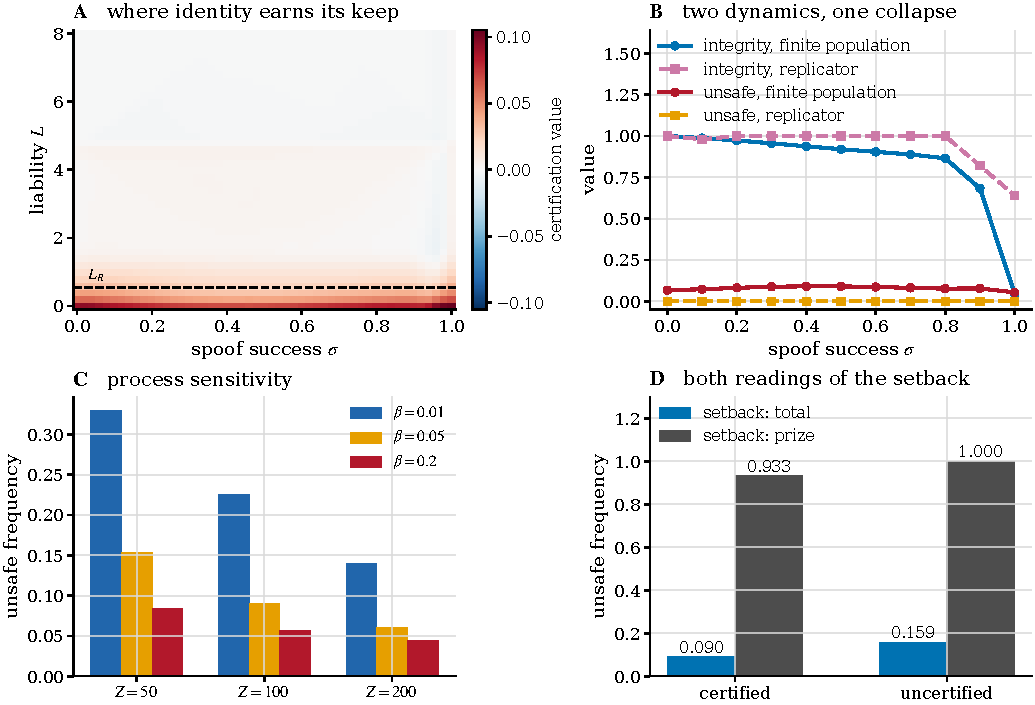
\includegraphics[width=\linewidth]{figures/fig09_robustness.pdf}
\caption{\textbf{Robustness.} \textbf{(A)} Certification value over spoof
success and liability; the dashed line is $L_R$. The instrument earns its keep
almost entirely below it. \textbf{(B)} The finite-population and replicator
readings along the spoof sweep: they agree on the collapse of attestation
integrity and disagree on the level of unsafe frequency, which is the finding
of Section~\ref{sec:exclusion}. \textbf{(C)} Population size and selection
intensity. \textbf{(D)} Both readings of the setback clause.}
\label{fig:robustness}
\end{figure}

\input{robustness_generated}

\section{Discussion}
\label{sec:discussion}

Three of our results bear directly on decisions being made now.

\paragraph{Attestation should be specified with its conduct rule, not without
it.} Standards work on agent
identity~\citep{a2a2026spec,xu2026agentdid,grogan2025agentfacts,otsuka2026aiidentity}
concentrates on the verification problem: how to bind a credential to an agent,
how to check it, how to revoke it. Our results say the verification problem is the easier half.
Equation~\eqref{eq:sigmastar} shows that what a club does with a verified
partner determines how much forgery the credential survives, and
Proposition~\ref{prop:exclusion} shows that what it does with an unverified one
determines the entire harm profile of the ecosystem. A credential specification
that leaves conduct to the market has left the load-bearing part
undefined~\citep{hadfieldmenell2019incomplete}.

\paragraph{Measure attestation integrity, not conduct.} Section~\ref{sec:channels}
shows a regime whose unsafe frequency is stable at about $0.06$ across
configurations whose attestation integrity ranges from $0.05$ to $0.94$.
Conduct monitoring cannot distinguish a certification system that works from
one that has been completely hollowed out by mimics, because a mimic
behaves.
The quantity to instrument is the posterior that a passed credential is
genuine, which requires sampling and independently re-verifying credentials
rather than observing outcomes. Section~\ref{sec:mimicry} makes the point
sharper: the healthier the interaction structure, the larger the share of
residual risk that conduct monitoring is blind to, because clustering removes
exploitation and leaves impersonation untouched. A regime that has invested
successfully in provider-scoped platforms has thereby made credential auditing
more important, not less.

\paragraph{Federate early, because the incentive decays.} The exclusion rent
falls from $30.4$ to $2.5$ as the market fragments from one provider to eight,
while the safety cost of non-federation rises from $0$ to $0.875$. The window
in which a dominant provider can be induced to accept mutual recognition is
therefore early, and the argument for it becomes strongest exactly when the
party who must agree has least to gain.

\paragraph{On the exclusion result.} We want to be careful about what
Observation~\ref{prop:bistable} and Proposition~\ref{prop:exclusion} do and do not
say. They do not say that certification is bad. Under rare mutation it roughly
halves
the unsafe frequency, and below $L_R$ it is the only instrument that works at
all. They say that its benefit is robustness rather than level, and that its
cost is a barrier rather than a harm~\citep{leland1979quacks}. A settled certified
market is exactly as safe as a settled uncertified one and poorer by its dues,
while a compliant outsider is charged $30.36$ despite conduct nobody objects
to. Whether that trade
is worth making depends on how often the market is knocked out of safety and
on how many participants sit outside the club, neither of which the model can
settle and both of which are measurable in a deployed system. What the model
does settle is that the trade cannot be avoided by asking clubs to be gentle
towards outsiders: that policy has spoof threshold zero without a fine. A
sufficiently large fine can restore resistance at fixed $\sigma$, but it cannot
give the gentle club a reason to exist (Corollary~\ref{cor:rescue}).

\paragraph{On multistability.} The methodological point generalises past this
model. Multistable evolutionary dynamics are
common~\citep{hofbauer1998evolutionary,hofbauer2003evolutionary,sandholm2010population},
and so is the practice of summarising a population by a single averaged
state~\citep{perc2017statphys}, and summarising one
by a basin-weighted mean state is a natural thing to do. Any observable that is
bilinear in the state, which includes every population average of a pairwise
quantity, must not be evaluated there: the mean of two pure regimes carries
cross-terms that neither regime contains. In our case that error turned a safe
ecosystem into one with an unsafe frequency of $0.368$ and manufactured a
boundary carrying $47.5\%$ of all encounters where the true figure is zero.

\subsection{Limitations}
\label{sec:limitations}

The interaction layer is a two-player reduced race with four designs, inherited
deliberately and without modification, so that every effect we report is
attributable to the identity layer rather than to a change in the underlying
game, and it is not a model of any particular deployment. The reduction to four designs
means the conduct space is coarse; a richer conduct space would allow
intermediate out-group policies that our scan cannot represent, and the sharp
zero-or-one structure of Table~\ref{tab:outgroup} would likely soften into a
frontier. We expect the direction of the trade to survive, since it follows
from Equation~\eqref{eq:sigmastar}, but not the exact numbers.

Verification is a single Bernoulli draw with a fixed $\sigma$, identical across
agents. A real attestation system has heterogeneous verifiers, revocation and
reputation carried between encounters in the manner of indirect
reciprocity~\citep{santos2018social}, where the threshold a reputation must
clear is itself under selection~\citep{yue2025reputation}. It may also face
adaptive forgers who
improve their forgeries as detection improves, as demonstrated for watermark
stealing~\citep{jovanovic2024watermarkstealing}. The last of these is the most
consequential omission: our $\sigma$ is exogenous, and an arms race in which
$\sigma$ responds to enforcement would change the comparative statics of
Section~\ref{sec:fines}.

Assortment is modelled as self-encounter probability, the standard reduction,
which conflates meeting one's own design with meeting one's own provider. A
network model in which providers are communities of many designs would separate
them, and the nucleation threshold would then depend on the community structure
rather than on a scalar.

Finally, the two dynamics we report answer two questions and neither is a
description of a running market. Actual agent ecosystems are neither
monomorphic nor sitting at a replicator rest point, and they are not, in
general, in either of the two dominant regimes of
Observation~\ref{prop:bistable}. Which of our two readings is the better guide
depends on how often the ecosystem is perturbed: the small-mutation reading
governs a market that is repeatedly knocked off its equilibrium, and the
replicator reading a market left alone. A model with an explicit perturbation
rate would interpolate between them and would be the natural next step.

One consequence of the multistability is worth naming as a limitation rather
than a result. The uniform-start sample does not estimate the basin of the
targeted unsafe rest face, and the $64$ perturbations around one deterministic
start establish only local numerical robustness, so the realised share of
cross-boundary states is unknown. Proposition~\ref{prop:exclusion} therefore measures the barrier off
the dominant equilibrium path, as the payoff a compliant entrant would
receive. That is the relevant quantity for entry, but the model predicts
neither that rest face's basin share nor the realised volume of
cross-boundary harm when certified and uncertified regimes coexist.

\section{Conclusion}
\label{sec:conclusion}

We made a forgeable identity badge a strategic variable in an evolutionary AI
race and characterised the resulting dynamics in closed form. Identity is the
instrument of last resort: below the reciprocity threshold of the race no
unbadged population holds safe play, and above it the identity layer is nearly
worthless. A club's resistance to forgery is set by its in-group conduct, and
conditional cooperation buys more than twice the tolerance of unconditional
trust. Fines cannot substitute for detection, because the protective fine
diverges as forgeries become undetectable, and in an agent economy detection is
technological rather than budgetary. No badge by itself starts a club from
anarchy without assortment,
and none rebuilds one after collapse. Mimics hollow out the credential before
exploiters degrade the conduct, so a monitoring regime that watches behaviour
sees nothing wrong while the mark stops meaning anything.

The result that reframes the rest concerns what certification is worth once a
market has settled. The replicator flow is multistable: two measure-dominant
safe faces coexist with a numerically robust unsafe badge-mixed rest face
revealed by targeted initialization. This targeted result is neither a basin
volume estimate nor evidence of a third isolated attractor. A
settled certified market is therefore no safer than an uncertified one and
poorer by exactly its dues; what certification buys is robustness, the
protection of a safe market against being knocked out of safety, which is why
it shows up under rare mutation and not at a rest point. Its cost is a
barrier: a compliant outsider that behaves exactly as club members do is
charged $30.36$ for carrying no badge. That toll is not incidental. It is the
only conduct under which the club survives forgery at all, since a club that
is safe towards outsiders has spoof threshold zero without a fine. A large
fine can restore its resistance at a fixed spoof rate, but not its evolutionary
purpose, and no finite fine substitutes for detection as $\sigma\to1$.
Certification and exclusion are the same mechanism, and a governance regime
that adopts the first has adopted the second whether or not it says so. The
instrument that escapes the trade is federation, which does not ask any club
to be gentle towards strangers but removes the category of stranger instead.


%% ===================================================================
%%  Elsevier / Chaos, Solitons & Fractals required declarations.
%%  The CRediT statement is NOT here: cas-sc builds it from the
%%  \credit{} commands in the front matter and \printcredits emits it,
%%  so edit the roles in _front.tex.
%% ===================================================================

\section*{Declaration of competing interest}

The authors declare that they have no known competing financial interests or
personal relationships that could have appeared to influence the work reported
in this paper.

\section*{Funding}

This research did not receive any specific grant from funding agencies in the
public, commercial, or not-for-profit sectors.

\section*{Data availability}

\begin{sloppypar}
The code, machine-readable results, generated tables and figures supporting
this article are deposited in the public repository at
\url{https://github.com/trungkiet2005/greenbeard-tag}. Every scalar quoted in
this manuscript is regenerated by \texttt{scripts/run\_analysis.py}
and \texttt{scripts/run\_robustness.py} into \texttt{results/};
\texttt{scripts/check\_numbers.py} then pins each quoted value to the results
key it came from, asserts that the value it pins occurs in the manuscript
source, and exits non-zero on any drift. Every figure is rendered by
\texttt{scripts/make\_figures.py} and checked for layout collisions by the
accompanying test suite. The interaction and identity layers carry no
simulation: the race is evaluated exactly over the horizon law, and the
handshake of Equation~\eqref{eq:handshake} is an exact four-term expectation.
The sampled quantities are the basin distribution and the explicitly separate
targeted perturbation probe of the replicator flow, described in
Section~\ref{sec:dynamics}. The closed-form spoof threshold of
Equation~\eqref{eq:sigmastar} is verified against brute-force root-finding on
the exact payoff matrices across dues, fines and liabilities; the remaining
closed forms are verified as invasion boundaries at the reported parameter
values.
\end{sloppypar}

\section*{Declaration of generative AI and AI-assisted technologies in the
manuscript preparation process}

During the preparation of this work the authors used Anthropic's Claude through
the Claude Code command-line interface and OpenAI Codex to assist with drafting
and editing prose; inspecting and revising LaTeX and bibliography files;
reviewing and revising analysis and theory code, validation checks and tests;
and developing deterministic plotting, build, packaging and reproducibility
tooling. All numerical values reported in the manuscript were checked against
or regenerated from deterministic, version-controlled scientific code, and all
submitted figures were rendered deterministically from model outputs and data
by that code. No generative image is included in the submission. The authors
reviewed and edited all tool-assisted output, reran the analysis and test
suites, reproduced the reported results, and take full responsibility for the
content of the published article.

\printcredits

\appendix
\renewcommand{\thesection}{Appendix~\Alph{section}}

\section{Proofs}
\label{app:proofs}

\begin{proof}[Proof of Proposition~\ref{prop:reciprocity}]
Against a \CS{} resident at $r=0$, the private payoff of a rare \CAS{} mutant is
$P(\CAS, \CS) = A(\CAS, \CS) - L\,M(\CAS, \CS)$ and the resident earns
$P(\CS,\CS)$. The difference is affine in $L$ with slope
$-[M(\CAS,\CS) - M(\CS,\CS)] < 0$, so it is positive exactly below the ratio
in Equation~\eqref{eq:LR}. With assortment, the exact difference against the
canonical safe resident is the joint expression in Equation~\eqref{eq:jointfirststrike};
the two intercepts cannot be combined into a rectangle. For the general statement, a safe unbadged resident
plays a safe design in self-play; since badges are absent, every check fails
and only $s_{\mathrm{out}}$ is ever executed, so the resident is behaviourally
one of $(\mathsf{N}, \cdot, \AS)$ or $(\mathsf{N}, \cdot, \CS)$. With
assortment $r$, the mutant meets itself with probability $r$, so the invasion
calculation above gives its advantage over a $(\mathsf{N},\cdot,\CS)$
resident at $L = 0$ as
$r\,A(\CAS,\CAS) + (1-r)\,A(\CAS,\CS) - A(\CS,\CS)$, which is affine and
decreasing in $r$ and vanishes at Equation~\eqref{eq:rdagger}. The same
calculation against a $(\mathsf{N},\cdot,\AS)$ resident gives
$42.77 - 74.57\,r$, which vanishes only at $r = 0.574$, so the
$(\mathsf{N},\cdot,\CS)$ residents are the binding ones and $r^{\dagger}$ is
the smaller of the two roots. The invasion of $(\mathsf{N}, \CAS, \CAS)$ against
each of the eight such residents is verified directly on the exact matrices at
$r = 0$, and the four $(\mathsf{N}, \cdot, \CS)$ residents are verified to
resist at the baseline $r = 0.1$.
\end{proof}

\begin{proof}[Proof of Proposition~\ref{prop:spoof}]
In a monomorphic club, a rare unconditional forger $(\mathsf{F}, w, w)$ meets
club members. Its badge passes with probability $\sigma$, in which case the
member plays $u$; otherwise the member plays $v$. The forger plays $w$
regardless. Its payoff is therefore
$\sigma P(w, u) + (1-\sigma) P(w, v) - \kappa_f - (1-\sigma)\rho$ and the
resident earns $P(u,u) - \kappa_g$. Both are affine in $\sigma$; equating and
solving gives Equation~\eqref{eq:sigmastar} whenever
$D=P(w,u)-P(w,v)+\rho\neq0$. This $D$ is the slope of the forger's advantage:
for $D>0$ that advantage increases with $\sigma$ and the club resists below the
threshold; for $D<0$ it decreases and the inequality reverses. Finally,
$D=0$ exactly when $\rho=P(w,v)-P(w,u)$, in which case the advantage is
independent of $\sigma$ and no division is made.
\end{proof}

\begin{proof}[Proof of Proposition~\ref{prop:fines}]
Solve the same indifference condition for $\rho$ instead of $\sigma$. The
numerator of Equation~\eqref{eq:rhostar} is the forger's advantage at zero
fine, and the denominator $1 - \sigma$ is the probability that a fine is
levied. If the numerator is positive at $\sigma = 1$, that is if
$P(w,u) - \kappa_f > P(u,u) - \kappa_g$, then $\rho^{*} \to \infty$.
\end{proof}

\begin{proof}[Proof of Proposition~\ref{prop:futility}]
Let the resident be $(\mathsf{N}, w, w)$. Its conduct does not depend on the
focal badge, so it plays $w$ whatever the focal design carries. The focal
design's own check of the resident always fails, since the resident carries no
badge, so the focal plays $s_{\mathrm{out}}$. The encounter is therefore
$(s_{\mathrm{out}}, w)$ for both a certified and an unbadged focal design with
the same conduct pair, and the payoffs differ only by $\kappa_g$. Since
$\sigma$ enters only through the pass rate of a forged badge, which is not
present, the identity holds at every $\sigma$; the same argument gives
independence of $\rho$ and $L$ enters both sides identically. The conclusion
follows because at $r = 0$ a rare mutant meets only residents.
\end{proof}

\begin{proof}[Proof of Proposition~\ref{prop:nucleation}]
With assortment $r$, a rare club mutant meets itself with probability $r$ and
the resident otherwise. Its fitness is
$r[P(u,u) - \kappa_g] + (1-r)[P(v,w) - \kappa_g]$, since in a self-encounter
both badges pass and both play $u$, while against the unbadged resident the
club plays $v$ and the resident plays $w$. The resident earns $P(w,w)$.
Rearranging the inequality gives Equation~\eqref{eq:rstar}.
\end{proof}

\begin{proof}[Proof of Proposition~\ref{prop:mimicry}]
The mimic $(\mathsf{F}, u, v)$ in a club population always sees the genuine
resident badge pass and therefore plays $u$. The resident plays $u$ towards
the mimic when its forged badge passes and $v$ when it does not.
Its expected payoff is $\sigma P(u,u) + (1-\sigma) P(u,v) - \kappa_f -
(1-\sigma)\rho$ against the resident's $P(u,u) - \kappa_g$. Solving for the
indifference point gives Equation~\eqref{eq:sigmam}. The mimic's threshold lies
below the exploiter's whenever the exploiter's conduct is worse in self-play
than the club's, which is what makes the exploiter pay a larger assortment
penalty.
\end{proof}

\begin{proof}[Proof of Proposition~\ref{prop:providers}]
Under symmetric shares, an agent of provider $k$ meets an agent of the same
provider with probability $1/K$, which equals
$\mathrm{HHI} = \sum_{k=1}^{K} (1/K)^{2} = 1/K$.
Within-provider checks pass and both play $u$; cross-provider checks
fail and both play $v$. Equation~\eqref{eq:hhi} is the resulting mixture. For
the baseline club, $U(\CS, \CS) = 0$ and $U(\CAS, \CAS) = 1$, giving
$U = 1 - \mathrm{HHI}$. Under federation every check passes and the mixture
collapses to $U(u,u)$.
\end{proof}

\begin{proof}[Proof of Proposition~\ref{prop:exclusion}]
Take $r = 0$, so that a rare entrant meets only members. A member of a
monomorphic club meets a member at every encounter, both checks pass and both
execute $u$, so its private payoff is $P(u,u) - \kappa_g$. The entrant carries
no badge, so every member's check of it fails and every member executes $v$,
while the entrant plays $u$ towards everybody by construction and therefore
earns $P(u,v)$ with no dues. The entry penalty is the difference,
$P(u,u) - \kappa_g - P(u,v)$, and the boundary unsafe frequency is $U(u,v)$,
neither of which involves $\sigma$. With $u = \CS$ and $v = \CAS$ this is
$59.00 - 2.00 - 26.64 = 30.36$ and $U(\CS, \CAS) = 0.461$; with $v = \CS$ the
encounter is $(\CS, \CS)$, so the penalty is $59.00 - 2.00 - 59.00 = -2.00$
and the boundary is safe. At the baseline assortment $r = 0.1$ the entrant's
own self-encounters lift its payoff and the penalty falls to $27.12$; the sign
and the ordering across out-group policies are unchanged.
\end{proof}

\begin{proof}[Proof of the harm decomposition of Section~\ref{sec:dynamics}]
The decomposition is an identity, not an approximation. Let $w_{ij}$ be the
probability of the ordered pair $(i,j)$ under the encounter law and let
$\mathcal{B}$ partition the ordered pairs by the badge status of the two seats.
Then $U = \sum_{ij} w_{ij} u(i,j) = \sum_{B \in \mathcal{B}} \sum_{(i,j) \in B}
w_{ij} u(i,j)$, so the block contributions sum to $U$ exactly. The zero entries
are exact in the model: a club member facing a club member executes
$(\CS, \CS)$, which contains no unsafe action, and the surviving unbadged
designs execute $(\CS, \CS)$ against each other for the same reason.
\end{proof}


\bibliographystyle{elsarticle-num-names}
\bibliography{refs}

\end{document}
